%\documentclass[12pt]{article}
\documentclass[12pt,titlepage,a4paper,oneside]{scrbook}
\usepackage{scrhack}
\usepackage[utf8x]{inputenc}
\usepackage{amsmath}
\usepackage{amssymb}
\usepackage{graphicx}
\usepackage{caption}
\usepackage[colorinlistoftodos]{todonotes}
\usepackage{subcaption}
\usepackage{geometry}
\usepackage{wrapfig}
\usepackage[strings]{underscore}
\usepackage{textcomp}
\usepackage{gensymb}
\usepackage{todonotes} 
 \geometry{
 a4paper,
 left=26.2mm,
 right=32.8mm,
 top=20mm,
 bottom=24mm
 }
\renewcommand{\familydefault}{\sfdefault}

%fancyheadings funktioniert nicht mehr mit der KOMA Script Klasse scrbook

\usepackage{wrapfig}

\usepackage[numbers,square,sort]{natbib}

% Mittels [H] können Bilder genau an einer Stelle positioniert werden
\usepackage{float}
\usepackage{hyperref}
% bewirkt das HyperLinks in der PDF nicht umrandet oder farbig sind
\hypersetup{colorlinks=false}

%Paket zur Erzeugung von Anführungszeichen durch \enquote{Text}
\usepackage[english]{babel}
%%\usepackage[babel, english=quotes]{csquotes}

%Verhindern, dass eine neue Seite für ein einzelnes Wort/Zeile verwendet wird
\clubpenalty = 10000 % schliesst Schusterjungen aus 
\widowpenalty = 10000 % schliesst Hurenkinder aus (keine Beleidigung, sondern wirklich ein Fachbegriff)
\linespread{1.25}
\setlength{\parindent}{0pt}
\setkomafont{chapter}{\normalfont\bfseries\fontsize{20}{15.5}\selectfont\scshape}
\setkomafont{section}{\normalfont\bfseries\fontsize{15}{15.5}\selectfont}
\setkomafont{subsection}{\normalfont\slshape\fontsize{12}{15.5}\selectfont}
\DeclareCaptionFont{xipt}{\fontsize{7.5}{13}\mdseries}
\usepackage[font=xipt,labelfont=bf]{caption}

\begin{document}
%!TEX root = ../Masterthesis.tex
\begin{titlepage}

\begin{center}
\begin{figure}[!ht]
	\centering
		\includegraphics[width=\textwidth]{images/th_color_bar.png}
\end{figure}
\end{center}
%Deutscher Titel
\begin{flushleft}
\begin{Large}
Masterthesis Medientechnolgie\\
\end{Large}
\vspace{0.5cm}
\begin{LARGE}
\textbf{RHOT-A real-time hand and object tracking system with low cost consumer grade hardware}
\end{LARGE}
\end{flushleft}
\vspace{1.0cm}
\begin{flushleft}
\begin{Large}
vorgelegt von\\ 
\vspace{0.3cm}
\begin{LARGE}
\textbf{Oliver Kalbfleisch} \\
\end{LARGE}
\end{Large}
\end{flushleft}
\vspace{2.0cm}
\begin{flushleft}
\begin{Large}
Erstgutachter: Prof. Dr. Arnulph Fuhrmann(TH Köln) \\[1.0em]
Zweitgutachter: Prof. Dr. Stefan Michael Grünvogel(TH Köln)
\end{Large}
\end{flushleft}
\vspace{1.5cm}
\begin{flushleft}
\begin{large}
Juni \the\year
\end{large}
\end{flushleft}
\begin{figure}[!ht]
\begin{flushright}

\includegraphics[width=0.25\textwidth]{images/TH_bottom_logo.png}
\end{flushright}
\end{figure}
\newpage
\setcounter{page}{1}
\pagenumbering{gobble}
\huge\textbf{Masterarbeit}\\\\
\large
Titel: RHOT Ein echtzeit Hand- und Objektrackingsystem basierend auf kostengünstiger Hardwarekomponenten\\
\textbf{Gutachter}:\\
	Prof. Dr. Arnulph Fuhrmann (TH Köln)\\
	Prof. Dr. Stefan Michael Grünvogel (TH Köln)\\
	\todo{übersetzen}
Zusammenfassung:\\ This paper will evaluate if it is possible to build a hand and object tracking system on low cost consumer grade hardware components. To keep system cost low, a set of Raspberry Pi's with the matching Camera is used for image acquiring an processing. These processing units are linked to a master unit which takes care of stereoscopic depth calculations, the position value processing and the final rendering of a hand and object model in digital space. Several forms of colored marker types are assessed for the prototype application and compared in terms of tracking precision and limiting factors in terms of haptic restrictions for the fingers. The final results show that it is possible to achieve a tracking system solution with the used hardware components that has a suitable tracking update frequency and precision.\\
\textbf{Stichwörter}: Echtzeit,Inverse Kinematik, Hand-tracking, color-tracking,Objekt-tracking, günstig)\\
\textbf{Sperrvermerk}: (optional) Die Einsicht in diese Arbeit ist bis zum TT. Monat JJJJ gesperrt.\\
\textbf{Datum}: TT. Monat JJJJ\\
\newpage
\huge \textbf{Masters Thesis}\\\\
\large
\textbf{Title}: RHOT A real time hand and object tracking system with low cost consumer grade\\
\textbf{Reviewers}:\\
	Prof. Dr. Arnulph Fuhrmann (TH Köln)\\
	Prof. Dr. Stefan Michael Grünvogel (TH Köln)\\
\textbf{Abstract}: \\This paper will evaluate if it is possible to build a hand and object tracking system on low cost consumer grade hardware components. To keep system cost low, a set of Raspberry Pi's with the matching Camera is used for image acquiring an processing. These processing units are linked to a master unit which takes care of stereoscopic depth calculations, the position value processing and the final rendering of a hand and object model in digital space. Several forms of colored marker types are assessed for the prototype application and compared in terms of tracking precision and limiting factors in terms of haptic restrictions for the fingers. The final results show that it is possible to achieve a tracking system solution with the used hardware components that has a suitable tracking update frequency and precision.\\
\textbf{Keywords}: Hand-tracking, Object-tracking, inverse kineamtics, low-cost, realtime \\
\textbf{Date}: 29 June 2018\\

\end{titlepage}

\tableofcontents
\setcounter{page}{1}
\newpage
\input{./chapter/Introduction}
\newpage
\newpage

\chapter{Description of the hand in digital space}
\label{sec:Description_of_hand_in_digital_space}
Tracking of the human hand has always been a challenging problem. In comparison to other larger body parts like the arm or the head, the human hand itself contains a large variety of smaller parts, namely bones and muscles. These components have to be taken into account when trying to replicate the natural motion of the hand in digital space.
\section{Physiological structure of the human hand}
\label{sec:Physiological_structure_of_the_human_hand}
Lee and Kuni \citep{LEE.1995} describe the human hand as "an articulated structure with about 30 degrees of freedom [which] changes shape in various ways by its joint movements."
\begin{figure}[H]
	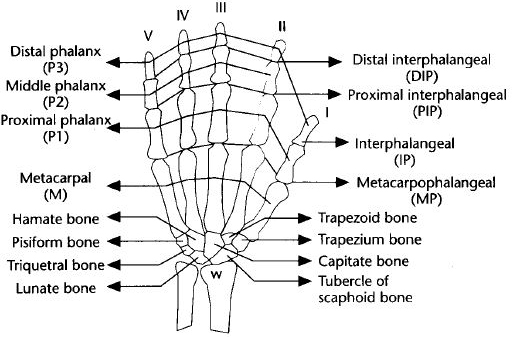
\includegraphics[scale=0.8]{images/hand.jpg}
	\label{Handstructure} 
	\caption{Bone structure of the human left hand (\cite{LEE.1995})}
\end{figure}
All of the hand components are connected to at least one neighboring component via a joint. The joints affect the position of the connected components. To describe the movement of the hand components, we can use the rotation angles of the joints to correlate to a specific position.
To do so, we define a local coordinate system for each of the exiting hand joints. By doing so, we achieve a sequence of rotations in the local coordinate systems of the joints. Such a sequence can then be used to describe a specific movement and/or position of a component.
Not all of the joints in the human hand have equal degrees of freedom. Their functionality can be classified in the amount of DOFs (Degrees of freedom)\cite{KOREIN.1985}
\begin{itemize}
\item 1 DOF \\
- A joint movement that can perform a \textbf{flexion} or \textbf{twist} in one direction
\item 2 DOF \\
- A joint movement that can perform \textbf{flexion} in more than one direction\\ (\textbf{directive})
\item 3 DOF\\
- A joint movement that permits simultaneous \textbf{directive} and \\ \textbf{twist} movements.(\textbf{spherical})
\end{itemize}
\begin{figure}[H]
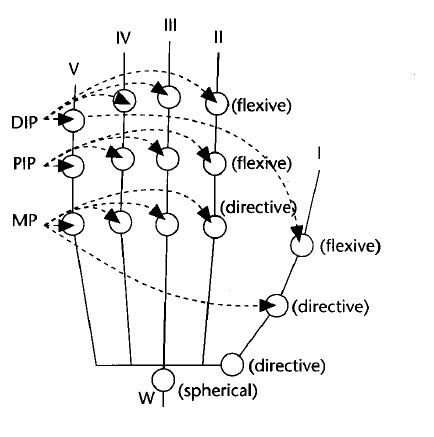
\includegraphics[scale=0.8]{images/Hand_DOFs.JPG} 
\caption{Representation of the DOFs of the human hand}
\label{dof_image} 
\end{figure}
When looking at the DOF's displayed in Figure \ref{dof_image}, each finger (II-V) sums up to 4 DOF's and the thumb to 5 DOF's. Also considering 6 DOFs for the rotation and position of the whole and itself, the result gets us to 27 DOF's  for the human hand.
\subsection{Constraints in hand motion}
A full usage of all the declared DOFs would lead to al large amount of possible combinations. Since the hand is not only made up of bones but also muscles and the skin, we can impose some constraints \cite{Badler.1987,Pavlovic.1997} to the movement of the joints. Ling, Wu and Huang(\cite{LIN.2000}) proposed following classification for the constraints:
\newpage
\begin{itemize}
\item \textbf{Type I constraints}\\
	-A constraint that limits the range of finger motions based on hand anatomy
	\item \textbf{Type II constraints}\\
	- A constraint that the position of the joints during finger movement
	\item \textbf{Type III constraints\\}
	-A constraint that limits position based on natural hand motions
\end{itemize} 
The \textbf{Type I} and \textbf{Type II} constraints rely on the physiological and mechanical properties of the human hand.\textbf{Type III} constraints are results of common and natural
movements and can be differing form person to person. As these movements are to some degree similar for everyone, a broad grouping can be applied. The curling of the fingers at the sane time when forming a fist is way more natural than curling each finger by itself. Here the motion of the hand is quite similar between different persons, but the constraints cannot be described in a mathematical form. 
 A \textbf{Type I} constraint example would be that the position of the fingertip is limited by the length of the other finger segments and thereby can only reach as far as the combined length.\\An example for \textbf{Type II} constraints would be that, for your fingertip to touch your hand palm, all joints in the finger have to be bend to achieve this position.
The following inequalities can be used to describe these constraints:
\textbf{Type I:}
\begin{equation}
\begin{split}
0\degree&\leq \Theta _{MP\_flex} \leq 90\degree\\
0\degree&\leq \Theta _{PIP\_flex} \leq 110\degree\\
0\degree&\leq \Theta _{DIP\_flex} \leq 90\degree\\
-15\degree&\leq \Theta _{MP\_abduct/adduct} \leq 15\degree
\end{split}
\end{equation}
A further constraint that is specific to the middle finger is, that this fingers MP normally does not abduct and adduct much. Therefore we can infer an approximation and thereby remove 1 DOF from the model:
\begin{equation}
\Theta _{MP\_abduct/adduct}=0\degree
\end{equation}
The same behavior can be seen in the combination of hand parts labeled W(the connection point between hand and lower arm). This approximation also eliminates one DOF on the connected thumb:
\begin{equation}
\Theta _{W\_abduct/adduct}=0\degree
\end{equation}
Since the DIP,PIP and MP joints of our index, middle, ring, and little fingers only have 1 DOF for flexion, we can further assume that their motion is limited to movement in one plane. \\
\textbf{Type II:}
The \textbf{Type II} constraints can be split into interfinger and intrafinger constraints. Regarding intrafinger constraints between the joints of the same finger, human hand anatomy implies that to bend the DIP joints  on  either the index, middle, ring or little fingers,the corresponding PIP joints of thath finger must also be bent. The approximation for this relation\cite{Rijpkema.1991} can be described as :

\begin{equation}
\Theta _{DIP} =\frac{2}{3}\Theta _{PIP}
\end{equation}
Inter-finger constraints can be imposed between joints of adjacent fingers. Inter-finger constraints describe that the bending of an MP joint in the index finger forces the MP joint in the middle finger to bend as well.\\
 When combining the constraints described in the above equations, the starting number 21 DOF's of the human hand can be reduced to 15. Inequalities for these cases, obtained through empiric studies, can be found in \citep{LEE.1995}.\\
 \todo{maybe move hand model section to here?}
\section{Kinematics}
\label{kinematics}
 The preceding sections gave an overview of how we can describe a model of the human hand and introduced some limiting constraints. With the model and the constraints, we can now start to build a kinematic system for the animation of the model.
Kinematic systems contain so called \textit{kinematic chains}, which consist of a \textit{starting point} or \textit{root}, kinematic elements like \textit{joints}, \textit{links} and an \textit{endpoint}, also called \textit{end effector}. Applied to the human hand, the whole hand model represents the kinematic system. This system contains several \textit{kinematic chains}, namely the fingers of the hand with the fingertips being the \textit{end effectors} of each of these chains.
Each of these components has it's set of DOF's which can be described mathematically. The established convention for describing this kind of linked systems is the \textit{Denavit-Hartenberg} convention (D-H)\cite{Denavit.1955}. It was actually introduced in order to standardize the coordinate frames for spatial linkages in the field of robotics, but has since then been applied in other fields as well.\cite{Spong.2008}
\todo{Denavit Hartenberg formmulation for coordinate System definition and transformation}  
As we begin to move our hands, the states of the kinematic chains begin to change. Joint angles and end effector positions are modified until the end position is reached. To represent the new position and angle data set of our physical hand with our kinematic system, two major paths for achieving a solution can be taken.
 \subsection{Forward Kinematics}
 
 Forward
 \label{Forward Kinematics}  kinematics (FK) uses the knowledge of the new angles and positions after the application of known transformations to the kinematic chain. The data of the \textit{joints} and \textit{links} between the \textit{root} and the \textit{end effector} is then used to solve the problem of finding the \textit{end effector's} position.
We can denote the existing end effectors relative position to an origin as $ s_{1},...,s_{k}$. The $s_{i}$ position is the result of th combination of all the joint angles in the corresponding kinematic chain. Respectively, we define the target position of the end effectors as $t_{1},...,t_{i}$, with $t_{i}$ being the target position for the end effector $s_{i}$. The required positional change for the end effector can now be described as $e_{i}=t_{i}-s_{i}$. In systems with more than one end effector, like our hand system, the components can be written as vectors.
\begin{equation}
\label{fk components}
\begin{split}
\vec{\textbf{s}}&=(\textbf{s}_{1},...,\textbf{s}_{n})^{T}\\
\vec{\textbf{t}}&=(\textbf{t}_{1},...,\textbf{t}_{n})^{T}\\
\vec{\textbf{e}}&= \vec{\textbf{t}}-\vec{\textbf{s}}\\
\end{split}
\end{equation}
As the vector components of $\vec{\textbf{s}}$ are results of the chain joint angles $\theta_{1},...,\theta_{n}$ and therefore are effected by them, we define 
\begin{equation}
\label{forward kinematic solution}
\begin{split}
\vec{\textbf{s}_{i}}&=f_{i}(\pmb{\theta})\\
\vec{\textbf{s}}&=f(\pmb{\theta})\\
\end{split}
\end{equation}
\\With $\pmb{\theta}$ being the column vector $\pmb{\theta}=(\theta_{1},...,\theta_{n})^{T}$.The second vector equation displayed in (\ref{forward kinematic solution}) is also called the \textit{Forward Kinematics}(FK) solution.
\\The advantage of an FK solution is that there is always an unique solution to the problem. In consequence, this approach is commonly used in the field of robotics, where the information on the chain elements is easily available.
The tracking of the human hand and all if its chain components is rather complicated.Therefore a solution which takes a known position of the \textit{end effector} and calculates the parameters for the rest of the chain would be more desirable.

 \subsection{Inverse kinematics}
 \label{inverse kinematics}
\begin{quote}"Inverse Kinematics (IK) is a method for computing the posture via estimating each individual degree of freedom in order to satisfy a given task" \cite{AndreasAristidouandJoanLasenby.2009}\end{quote}
The concept of \textit{Inverse Kinematics}  (IK) already describes it's principle in it's name. It takes the reversed approach in comparison to the FK principle in chapter \ref{Forward Kinematics}. Instead of knowing the states of the chain elements and calculating the resulting position of the \textit{end effector}, we take the position of the \textit{end effector} and try to retrieve the possible states of the other chain elements. 
\begin{equation}
\label{ik problem formula}
\pmb{\theta}=f^{-1}(\vec{\textbf{s}_{d}})
\end{equation}
The result of this equation is the vector $\pmb{\theta}$ for which the values of $\vec{\textbf{s}}$ coincide to the desired configuration $\vec{\textbf{s}_{d}}$. In the case of an optimal result, this configuration would have the same position values as the target positions.\\ The main problem with this method occurs in the calulaton of the $f^{-1}$ function, due to it beeing a highly non linear operator which is not easily invertible.The approaches that \cite{AndreasAristidouandJoanLasenby.2009} describes to counter this problem will be displayed later on in this chapter.
In contrary to having a unique solution with the FK approach, the IK approach can end at the point of not finding a suitable solution. Figure \ref{IkSolutions} displays three possible outcomes for the IK approach.
\begin{figure}[H]
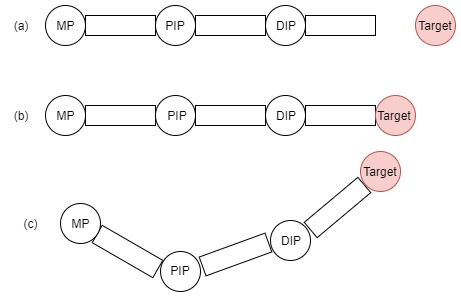
\includegraphics[scale=0.6]{images/Ik_figure.jpg}
\caption{Possible solution for an IK problem of a human finger:\\(a)The given target position of the end effector can not be reached. (b) The given target can only be reached by one solution.(c) The target position can be reached with multiple different solutions.}
\label{IkSolutions}
\end{figure}
\subsection{Jacobian-based methods}
\subsubsection{Jacobian inverse}
One common approach to solve the IK problem is the utilization of a Jacobian Matrix and an iterative calculation process. This matrix contains the partial derivatives of the chain systems relative to the end effector \textbf{s}. When using the Jacobian, a linear approximation  of the IK problem will be applied for solving. The approximation's components model the end effector's relative movement to changes in transitions of the systems link translations and joint angles. Therefore, the resulting function is dependent on the joint angles $\pmb{\theta}$ values and can be defined as
\begin{equation}
\label{Jacobian definition}
J(\pmb{\theta})_{ij}=\left(\frac{\partial\textbf{s}_{i}}{\partial\theta_{j}}\right)_{ij}
\end{equation}
with \textit{i}=1,...,k and \textit{j}= 1,...,n.
Further readings on methods for the calculation of Jacobian matrices can be found in \cite{Orin.1984}. Based on definition (\ref{Jacobian definition}), an entry for the j-th rotational joint would be calculated as follows:
\begin{equation}
\label{Jacobian entry calc}
\frac{\partial \textbf{s}_{i}}{\partial \theta_{j}}= \textbf{v}_{j}\times(\textbf{s}_{i}-\textbf{p}_{j})
\end{equation}
where $\textbf{p}_{j}$ is the position of the joint, and $\textbf{v}_{j}$ is the unit vector pointing along the current axis of rotation for the joint.
Taking the derivative of definition (\ref{forward kinematic solution}) with respect to time gives the basic equation for forward kinematics that describes the velocities of the end effectors:
\begin{equation}
\label{fk derivate}
\dot{\vec{\pmb{s}}}=\pmb{J}\pmb{(\theta)}\dot{\pmb{\theta}}
\end{equation}
\\ Now having all the values for the angles, the \textit{end effector} position and the target positions, we can compute the resulting Jacobian matrix.
Thereafter we seek an update value $\Delta\pmb{\theta}$ for incrementing the current joint values:
\begin{equation}
\label{theta calc}
\pmb{\theta}_{new}=\pmb{\theta}_{curr}+\Delta\pmb{\theta}
\end{equation}
The idea here is that the  chosen value for $\Delta\pmb{\theta}$ should lead to the resulting $\Delta\pmb{\vec{s}}$ being approximately equal to $\vec{\textbf{e}}$ from (\ref{fk components}). The $\vec{\textbf{e}}$ can be approximated by:
\begin{equation}
\label{delta s approx}
\Delta\pmb{\vec{s}}\approx \pmb{J(\theta_{curr})}\Delta\pmb{\theta}
\end{equation}
Using this approximation  we can reformulate the FK problem as $\pmb{}\vec{\pmb{e}}=J\Delta\pmb{\theta}$ and therefore our inverse kinematics problem form \ref{ik problem formula} can be expressed as $ \Delta\pmb{\theta}=J^{-1}\vec{\pmb{e}}$. \\The problem we run into with this solution is the construction of the inverse Jacobian matrix. The Jacobian J may not be square or invertible. In the case of it beeing invertible , the result may only work inferiorly because of it being nearly singular. Being singular means that no change in joint angle values may achieve the desired end effector position as an outcome.
\subsubsection{Jacobian transpose}
One approach to calculating the value of $\Delta\pmb{\theta}$ without having to calculate the inverse of \textbf{J} is done by replacing the inverse with the transpose of \textbf{J}.
\begin{equation}
\label{delta theta transpose}
\Delta\pmb{\theta}=\alpha \pmb{J}^{T}\vec{\pmb{e}}
\end{equation}
Of course the transpose and the inverse of \textbf{J} are not the same thing. When using the theorems displayed in \cite{DavidE.Orin.1984,Wolovich.1984} we can show that: 
\begin{equation}
\label{transpose show}
\langle JJ^{T}\vec{\pmb{e}},\vec{\pmb{e}}\rangle=\langle J^{T}\vec{\pmb{e}},J^{T}\vec{\pmb{e}}\rangle=\|J^{T}\vec{\pmb{e}}\|\geq 0
\end{equation}
Under a sufficiently small $\alpha>0$ the updated angles from \ref{theta calc} will change the end effector positions by approximately $\alpha JJ^{T}\vec{\pmb{e}}$. They also state that 
the value of $\alpha$ can be calculated by minimizing the new value of the error vector $\vec{\pmb{e}}$ after each update.
\begin{equation}
\label{transpose alpha}
\alpha=\frac{\langle\vec{\pmb{e}},JJ^{T}\vec{\pmb{e}}\rangle}{\langle JJ^{T}\vec{\pmb{e}},JJ^{T}\vec{\pmb{e}}\rangle}
\end{equation}
\subsubsection{Jacobian pseudo inverse}
Instead of calculating the normal inverse of the Jacoboian, which can lead to the problems described before, we can use the so called \textit{pseudo-inverse}\cite{Dahmen.2008} for the calculation. The \textit{pseudo inverse} is defined for all matrices J, even ones
which are not square or not of full row rank.
\begin{equation}
\label{pseudo inv def}
\Delta\pmb{\theta}=J^{\dagger}\vec{\pmb{e}}
\end{equation}

The \textit{pseudo inverse} represents the best possible solution for $ J\Delta\pmb{\theta}=\vec{\pmb{e}}$ in respect to least squares, but does suffer from instability near singularities. It has the property that the matrix $(I − J^{\dagger}J)$ performs a projection onto the null space of \textbf{J} . Therefore, for all vectors $\varphi, J(I −J^{\dagger}J)\varphi = 0$. Therefore $\Delta\pmb{\theta}$ can be set by
\begin{equation}
\Delta\pmb{\theta}=J^{\dagger}\vec{\pmb{e}}+(I-J^{\dagger}J)\varphi
\end{equation}
for any vector $\varphi$ and still obtain a value for $\Delta\theta$ which minimizes the value $ J\Delta\pmb{\theta} −\vec{\pmb{e}}$.The pseudo inverse of \textbf{J} can be derived as follows:
\begin{equation}
\begin{split}
\pmb{J}^{\dagger}&=(\pmb{J}^{T}\pmb{J})^{-1}\pmb{J}^{T}\\
\Delta\pmb{\theta}&=(\pmb{J}^{T}\pmb{J})^{-1}\pmb{J}^{T}\vec{\pmb{e}}\\
(\pmb{J}^{T}\pmb{J})\Delta\pmb{\theta}&=\pmb{J}^{T}\vec{\pmb{e}}\\
\end{split}
\end{equation}
Using $\vec{\pmb{y}}=\pmb{J}^{T}\vec{\pmb{e}}$, we can now solve the equation $(\pmb{J}^{T}\pmb{J})\Delta\pmb{\theta}=\vec{\pmb{y}}$

\subsection{Singular Value Decomposition}
The usage of a \textit{singular value decomposition} is another method of calculating the \textit{pseudo inverse} of a jacobian matrix. A singular value decomposition of \textbf{J} consists of expressing \textbf{J} in the form
\begin{equation}
\pmb{J} = \pmb{UDV^{T}}
\end{equation} 
For an \textit{m×n} Jacobian matrix, \textbf{U} is\textit{ m×m} and the columns are the eigenvectors of $JJ^{T}$. \textbf{D} is \textit{m×n}, and the entries are zero except along the diagonal where $d_{ii}=\sigma_{i}$ with $\pmb{\sigma_{i}}$ beeing the singular value and $\sigma 1\geq \sigma 2 \geq ...\geq \sigma m \geq 0$. Singular values are the non-negative square roots of the eigenvalues of $JJ^{T}$ and $ J^{T}J$.\textbf{V} is \textit{n×n} and the columns are the eigenvectors of $J^{J}J$.
The construction of the pseudo inverse is done as follows:
\begin{equation}
\pmb{J}^{\dagger} = \pmb{VD^{\dagger}U^{T}}
\end{equation} 
The pseudo-inverse of the diagonal matrix \textbf{D} is obtained by replacing each positive diagonal entry with it's reciprocal \cite{Golub.1965}.
\subsection{Damped Least Squares}
 The \textit{Dampened Least Squares} method is is applied for inverse kinematics as it avoids the singularity problems that can occur when using the pseudoinverse.It further provides a numerical stable method for selecting $\Delta\theta$. First occurences for inverse kinematics can be found in \cite{Wampler.1986,Nakamura.1986}.
Instead of finding the minimum for $\Delta\theta$ as a best solution for the equation displayed in \ref{fk components}, the goal of this method is to find the value that minimizes the following quantity with $\lambda \in \mathbb{R} $ as a dampening factor.
\begin{equation}
\parallel J\Delta\pmb{\theta}-\vec{\pmb{e}}\parallel^{2}+\lambda^{2}\parallel\Delta\pmb{\theta}\parallel^{2}
\end{equation}
which can be rewritten to the corresponding 
\begin{equation}
(\pmb{J}^{T}\pmb{J}+\lambda^{2}I)\Delta\pmb{\theta}=\pmb{J}^{T}\vec{\pmb{e}}
\end{equation}
and therefore 
\begin{equation}
\Delta\pmb{\theta}=(\pmb{J}^{T}\pmb{J}+\lambda^{2}I)^{-1}\pmb{J}^{T}\vec{\pmb{e}}
\end{equation}
The selection of a correct $\lambda$ value is essential for this method, small values of $\lambda$ give accurate solutions but low robustness to the occurrence of singular and near-singular configurations, while large  values of $\lambda$ result in low tracking accuracy even when a feasible and accurate solution would be possible\cite{Chiaverini.1994,AndreasAristidouandJoanLasenby.2009}.

\subsection{Newton Methods}
The Newton family of methods is based on a second order Taylor series expansion of the object function f(x):
\begin{equation}
f(x+\sigma)= f(x)+ [\bigtriangledown f(x)]^{T}\sigma + \frac{1}{2}\sigma^{T}H_{f}(x)\sigma
\end{equation}

where Hf(x) is the Hessian matrix. The downside of this approach is that the calculation of the Hessian matrix bares high computational cost for each iteration as a result of its complexity. Like the approximation of the Jacobian inverse, several attempts to lower the computational cost have benn made by utilizing an approximation of the Hessian matrix based on a function gradient value.
Since the Newton methods are posed as a minimization problem, they return smooth motion without erratic discontinuities.
The Newton methods also have the advantage that they do not suffer from singularity problems, such as that which occurs when finding the Jacobian Inverse.
<<<<<<< HEAD
\newpage
=======

>>>>>>> a57ff10d7afd7316e3ea8c75be34cac0a87d3b14
\subsection{FABRIK Algorithm}

 A more recent approach in the kinematics field is the \textbf{FABRIK} algorithm proposed by Aristidou and Lasenby\cite{Aristidou.2011}.As shown in section \ref{inverse kinematics}, these approaches all depend on computational intensive matrix operation like calculating an inverse and may have problems with matrix singularity.
\begin{wrapfigure}{r}{0.61\textwidth}
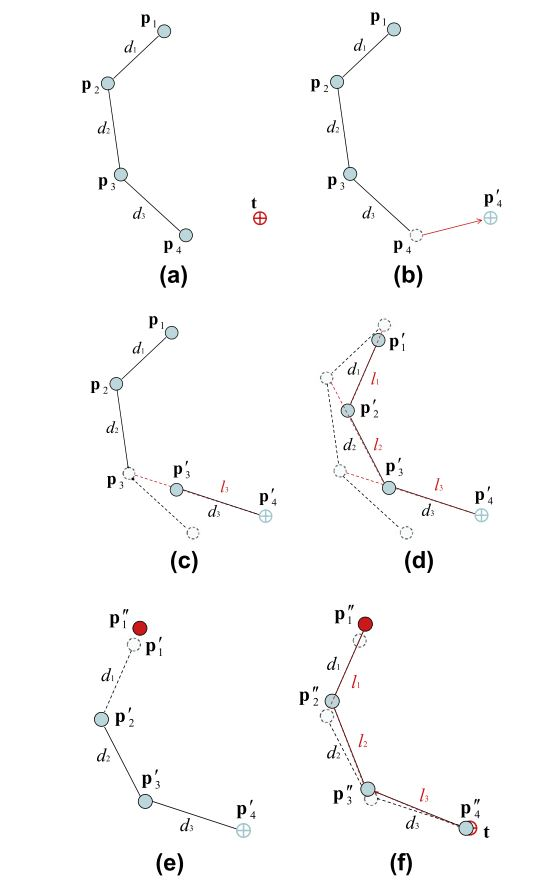
\includegraphics[scale=0.61]{images/FabrikIteration.jpg}
\caption{Forward and backward calculation steps for one iteration of the \textbf{FABRIK}algorithm.(a) initial position of the system.(b)End effector is moved to target position.(c) Deterimne position of next joint on constructed line.(d)repeat until root is reached. (e)move root joint to initial position. (f) repeat calculation in reverse direction \cite{Aristidou.2011} }
\label{Fabrik_Iteration}
\end{wrapfigure}

The \textbf{FABRIK} algorithm does not depend on these matrix operations as is solves for the position of a point on a line to retrieve the new joint positions. This is done in an forward and also inverse solving approach, iterating these steps until the calculated position converges towards the target position from the tracking data.
Figure \ref{Fabrik_Iteration} illustrates the steps that are contained in one iteration step.
The chain joints are denoted as $\textbf{p}_{\textit{i}}$ with the distance $\textbf{d}_{i}$ being $|\textbf{p}_{\textit{i+1}}-\textbf{p}_{\textit{i}}|$. The target point for the end effector is denoted as \textbf{t}. Step \textbf{(a)} displays the starting point of the iteration. The joint positions are taken from either a previous iteration or from an initial calibration. 
But before calculations can begin, the algorithm has to check whether the intended target point \textbf{t} is reachable for the end effector. This is done by measuring the distance between the root of the kinematic chain and the target point \textbf{t}. This value is then compared with the sum of the distances $\textbf{d}_{i}$.
\begin{equation}
 dist_{t,d_{1}}< \sum_{k=1}^{i}{d_{i}}
\end{equation}The inverse calculation step is the first step, which is displayed in \textbf{(b)} and \textbf{(c)}.The calculation is started at the end effector, moving to the root of the chain. 
If the summed distance is greater, then the \textbf{t} is within the reach of the system and the calculation can continue, otherwise the calculation has to be aborted and the error has to be manged otherwise.
Assuming this requirement to be met, we can now begin with the first calculation. Therefore we assume that the new position $\textbf{p}_{n}^{'}$ with n=4,...,1 is equal to \textbf{t}.
\begin{equation}
 \textbf{p}_{n}^{'}=\textbf{t}
\end{equation}
From this new point, we can construct a line that goes through $\textbf{p}_{n}^{'}$ and $\textbf{p}_{n-1}$.
\begin{equation}
\begin{split}
A&=\textbf{p}_{n}^{'}\\
B&=\textbf{p}_{n-1}\\
\textbf{l}_{n-1}&=\overline{AB}\\
\end{split}
\end{equation}
The resulting position of the new $\textbf{p}_{n-1}^{'}$ point is located in this line with the distance of $\textbf{d}_{n-1}$ from $\textbf{p}_{n}^{'}$ (see \textbf{(c)}).
\begin{equation}
\textbf{p}_{n-1}^{'}= \textbf{p}_{n}^{'}+ \left(\frac{\overline{AB}}{|\overline{AB}|}\cdot\textbf{d}_{n-1}\right)
\end{equation}
Consecutively, this is done with the remaining joints until the root joint is reached(see \textbf{(d)}).
This finishes the first halve of the iteration step.With the calculated positions, we now perform a forward calculation, starting from the root until we reach the end effector. Since the root of the system normally does not move from it's initial position, we have to reset the root joint to this value before starting to calculate the new positions of the subsequent joints(see\textbf{(e)}).

Analogous to the procedure in the inverse step, we construct the lines between the points and determine the new position values of the joints. The end result of this step is shown in \textbf{(f)}. At this point, we can decide if the result position of the end effector is appropriate in comparison to the value of \textbf{t}. A simple threshold value for this case could be the position difference between these two points.
\todo{constraints adding for the algorithm}
\todo{review of algorithm capabilities}
\newpage
%!TEX root = ../Masterthesis.tex
\chapter{Tracking in real space}
The previous sections provided information on the structure of the human hand and how to represent it in the digital space. To apply the algorithms presented in Section \ref{kinematics} to our digital hand model, we need input data from our real world representative.
\section{General tracking technologies}
\label{General tracking technologies}
The methods for gaining positional data can be roughly categorized into two major groups, glove based methods and vision based methods. Glove based methods have already been in developement since the 1980's \cite{Bolt.1980} and have since then resulted in several solution attempts. Sturman and Zeltzer gave a survey on the exsisting tracking mehtods in their paper \cite{Sturman.1994}. They distinguish between two areas of tracking, first the 3D positional tracking of the hand (and also other bodyparts) without regard to the hands shape and secondly the tracking of the hand shape with glove technologies.These tracking technologies presented are still applied today in modern tracking solutions \cite{Welch.2002,Rolland.2001}. They account for solutions based in optical tracking based on marker detection, magnetic detection via measurements of an artificial magnetic field\cite{Raab.1979} and acoustic measurements via triangulation of ultrasonic pings.

\subsection{Optical tracking}
The components for an optical tracking systems are several cameras for object detection and some kind of tracking characteristic of the object to be tracked. These characteristics can be either artificially applied ones like active flashing infrared LED on key tracking positions of the body or infrared reflective markers. A series of cameras positioned around the tracking subject will then track these markers inside their visual fields. The second method uses a single camera to capture the silhouette image of the subject, which is analyzed to determine positions of the various parts of the body and user gestures.
The image data is supplied to special software which correlates the marker positions in the multiple viewpoints and uses the different lens perspectives to calculate a 3D coordinate for each marker. These image interpretation and correlation tasks require computationally costly operations. The marker tracking is also prone to errors through variation in lighting of the scene, material reflection properties and also marker occlusion as the trackers are moved. Also most of the systems rely on several tracking cameras for a complete coverage of the tracking space. This leads to a higher system complexity in terms of setup and calibration.
\begin{figure}[H]
\label{optic reflector tracking}
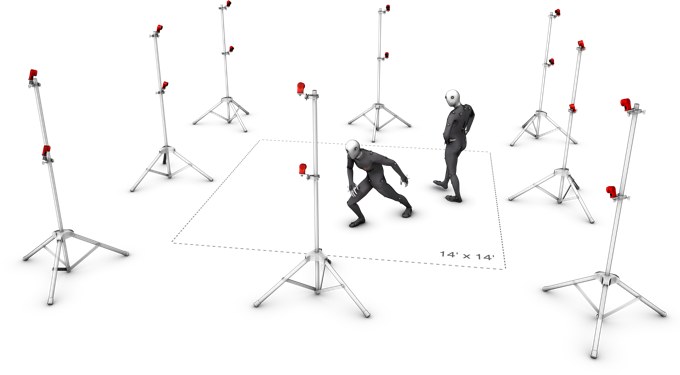
\includegraphics[scale=0.6]{images/flex13MocapVolume.png} 
\caption{Example for an optical tracking system with passive infrared reflector markers \cite{optitrack.2017}}
\end{figure}
\subsection{Magnetic tracking}
The usage of a magnetic field for position tracking is a relatively uncomplicated technique. The earth already provides us with a magnetic field to orient on. Similar to the optical trackers, magnet field sensors can be placed at key tracking positions. These sensors measure field strength in 3 orthogonal oriented axes to produce a 3D vector of the units orientation with respect to the excitation. As the earths magnetic field prone to changes based on geographical location, data corrections have to be applied to the measurements.Another solution is to generate an local magnetic field via a multi-coil source unit. The source unit coils are energized in sequence and the corresponding magnetic field vector is measured in the sensor unit. With three such excitation's, you can estimate the position and orientation of the sensor unit with respect to the source unit.T he downside of this technology is that ferromagnetic and conductive material in the surrounding environment will have an effect on the generated magnetic field. These distortion effects will form small unwanted secondary source units through the induction of small Foucault currents by the main sources magnetic field.
Magnetic fields have the property of having an inverse cubic falloff  as a function of distance from the source, which limits the range of operation for the system.
Position resolution in the radial direction from source to sensor depends on the gradient of the magnetic field strength, and thus the positional jitter grows as the fourth power of the separation distance.
In comparison to other tracking technologies, the magnetic field tracking solution has the convenience of not suffering from line of sight problems from tracker occlusion. The magnetic fields are capable of passing through the human body. Also the sensor size for measuring magnetic fields is rather small, giving the trackers a small volume. Furthermore, only one source unit is needed for the tracking of multiple sensor units.
\subsection{Accoustic tracking}
The principles of acoustic tracking are very similar to those of the optic tracking technologies. Instead of using lightwaves, the systems utilize acoustic pulses of ultrasonic wavelengths to time the time of flight between emitter and sensor for range measurement. To get a good measuring result from the systems, the used acoustic transducers have to be as omnidirectional as possible,so that the signal can be detected no matter how the emitter is positioned or oriented in the tracking volume. For the speakers to achieve a wide beam width, their size has to be small.
To be able to build the microphones into the tracker, they can only have active surfaces a few millimeters in diameter. This leads to a reduction in range as the efficiency of acoustic transducers is proportional to the active surface area. Also acoustic systems can have problems with ambient noises occluding the signal. This becomes even more critical when using such a system outdoors.Sound waves travel at a much slower speed than light waves which brings benefits and downsides with it. Sound waves can be reflected from objects, producing so echos which arrive at the receiving sensor at a later point in time. Here the slower speed can be beneficial as we can await the first sound occurrence to arrive at the sensor and filter out all later reflections from the data. The reflections of the previous pulse also have to be subsided before a new measurement can be made, lowering the update rates of the system. The air the sound waves travel through is also a limiting factor as humidity, air pressure and air currents can influence the traveling sound waves.In comparison to the optical systems, the acoustic systems are not as prone to occlusion errors since sound waves have a better ability to bend around obstacles than light waves.
Most of these downside can be adressed with a combination of these systems with another form of tracking like in \cite{Foxlin.1998}.
\section{Hand tracking Systems}
\label{hand-tracking_systems}
In comparison to the tracking of the whole human body, the tracking of the human hands with their maximum of 27 DoF's each in a small space is rather difficult to handle.
The systems that try to achieve this have to encounter several difficulties. Self occlusion also plays a great role in the system design, especially when working with only one tracking optical system for reduced complexity. Also these systems need to maintain a certain amount of processing speed for achieving a fluent reproduction of the captured motion. This demands the capability of processing large amounts of data in very short intervals. Most prototype testing for the described systems will be done in an controlled environment where the background is known. For a more widespread use, these systems need to be capable of registering the hand on an unrestricted background, which may have a wide range of patterns, color and lighting differences. Also human hand motion itself is quite fast, resulting in a higher frame rate demand for the tracking cameras.
The following section will describe different approaches to solve the aforementioned difficulties.

\subsection{Sensor based}
\label{Sensor based}
Tracking systems thath make use of sensors mounted to the hand via straps or a glove have alread been in use since the 1970's. First prototype glove systems included the Sayre Glove\cite{ThomasA.DeFanti.1977} and the Digital Entry Data Glove\cite{Grimes.1983}.
The Sayre glove is based off an idea of Richard Sayre. The system utilizes a light source and a photocell which are connected via a flexible tube. These components are mounted along each finger of the hand. The light that passes through the tube is influenced by the bending angle of the tube which corresponds to the finger bending.
a large bending angle of the finger induces a larger bending angle of the tube, reducing the intensity of the light that reaches the photo diode. The resulting voltage in the photocell can then be mapped to a specific bending angle of the finger.
The Digital Entry Data Glove was patented by Gary Grimes in 1983. Instead of using only one type of sensors for measurement, this glove based systems used several sensor types for different measurements.
Touch or proximity sensors were used for determining whether the user's thumb was touching another part of the hand or fingers. To measure the flexion of the joints in the thumb, index, and little finger four “ knuckle-bend sensors ” were used.
\begin{wrapfigure}[11]{r}{5cm}
\label{acceleglove}
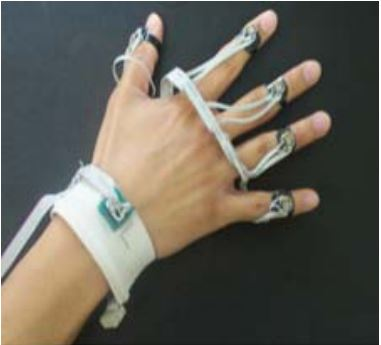
\includegraphics[scale=0.5]{images/acceleglove.JPG} 
\caption{Acceleglove system with the described sensor positions \cite{HernandezRebollar.2002}}
\end{wrapfigure}
To get measurements  for the tilting of the hand in respect to the horizontal plane two tilt sensors were mounted. Finally two inertial sensors for measuring the twisting of the forearm and the flexing of the wrist were utilized.This glove was intended for creating “ alphanumeric characters ” from hand positions. Recognition of hand signs was performed via a hard-wired circuitry, which mapped 80 unique combinations of sensor readings to a subset of the 96 printable ASCII characters.
These early systems only provided a limited amount of sensors and were rather unpractical in use. As they were developed to serve very specific applications,  they were used only briefly, and never commercialized.
Newer developements in this sector include \cite{Kuroda.2004,HernandezRebollar.2002,Majeau.2012}. The \textit{AcceleGlove} presented by \cite{HernandezRebollar.2002} consists of six dual-axis acelerometers, mounted on the fingers and the back of the palm, reporting position with respect to the gravitational vector. Sensors are placed on the back of the middle phalanges, on the back of the distal phalange of the thumb, and on the back of the palm.
Kuroda et al \cite{Kuroda.2004} introduced the \textit{StrinGlov}, which obtains full degrees of freedom of human hand using 24 Inductcoders and 9 contact sensors, and encodes hand postures into posture codes on its own DSP. The bending angles of the fingers are measured with the inductcoders. These sensors realte the finger movement to a change in magnetic flux induced by the movement of the sensor parts thath are attached to the finger. The sensor functionality is simular to the functionality of the light sensors from \cite{ThomasA.DeFanti.1977}. The 9 contact sensors, also based on magnetic fields,  are put on the fingertips and on the inside of the hand to be able to measure contact between two fingertips or the fingertips and the hand. The system furthermore benefits from simple structure, which leads to low production cost. 
Majeau et al \cite{Majeau.2012} propsed a systems that uses optical flexion sensors to determine the bending angles of the fingers. The opticcal flexion sensors consist of a LED, a Photodetector and an optical fibre. The LED emits light which travels through the optical fibres and the intensity that results as the output from the fibre end is measured by the Photosensor. This measuring principle also corresponds to the principle of \cite{ThomasA.DeFanti.1977}. Furthermore the system is also capable of measuring the abduction of two finger. Here the LED is mounted to one finger and the detector on the other. The optical fiber is run from the LED down the finger to the knuckle base and then up to the detector. When abducting the two fingers, the angle at the knuckle base changes, resulting in an intensity change at the detector through the loss of intensity at the curvature of the optic fiber.
The change in intensity of both measuring techniques can be mapped to corresponding hand movements.
Further readings on sensor based hand tracking systems can be found in \cite{Dipietro.2008,Sturman.1994}
\subsection{Appearance Based - Optical marker}
\label{Appearance Based Optical marker}
Optical approaches use properties of the human hand to hand to estimate the current position. The evaluation of the hand pose is usually split up into two steps. The first one is the registration of the "real" hand.\\
\begin{wrapfigure}[7]{r}{0.52\textwidth}
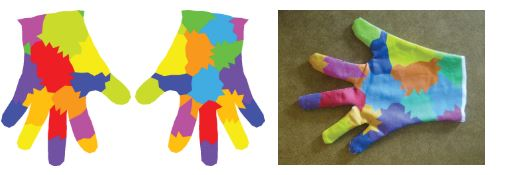
\includegraphics[scale=0.61]{images/wang_color_glove.JPG}
\caption{Color glove setup used by Wang and Popovic \cite{Wang.2009} }
\label{wang color glove}
\end{wrapfigure}
This is mostly done by at least one camera which is aimed at the hand, supplying a "continuous" data stream to the evaluation Software. In the section step, the evaluation software then tries to find key spots in the provided images. This data is then used for the search of the matching digital pose. The definition of these key spots can be achieved by several techniques.
An example is the usage of some kind of marking for finger segments as displayed in \cite{Duca.2007,Fredriksson.2008,Wang.2009}.
In the method described by Wang and Popovic \cite{Wang.2009},a specially colored glove is used. The glove is segmented into ten segments, colored randomly from a pool of ten distinct colors (see Figure \ref{wang color glove}).
\newpage
\begin{wrapfigure}[14]{r}{0.42\textwidth}
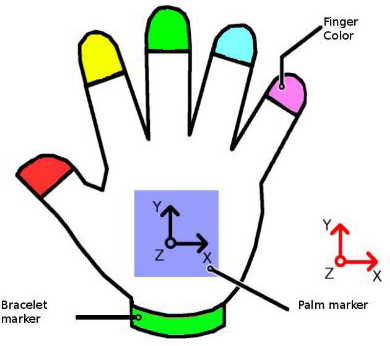
\includegraphics[scale=0.61]{images/fredrikkson_color_glove.JPG}
\caption{Color glove setup used by Fredriksson and Ryen \cite{Fredriksson.2008} }
\label{Fredriksson color glove}
\end{wrapfigure}

The pattern is created by selecting twenty seed triangles on a 3-D hand model that are maximally distant from each other. The remaining triangles are assigned into patches based on their distance to each of these seeds. Each patch is assigned one of the ten colors at random. The jagged boundaries between the patches are artifacts from the low triangle count of the used hand model.
Algortihms that use other characteristics for tracking like texture or shading \cite{LaGorce.2008} rely on an accurate pose from a previous frame to constrain the posture search in the current frame. When using bare hand pose estimation two different hand poses can map to similar images. This can lead to an inaccurate pose estimation and the breakdown of the algorithm if the wrong estimation is made.
The benefit of the color glove is that the unique patch pattern, hand poses always map to distinguishable images, simplifying the search process. Therefore it can effectively recover itself at each frame without the need of a previous frame.
With the colored glove as a tracking feature, the images from the camera are prepared for a database sampling step. The database that was used consisted of 18,000 finger configurations. 
A distance metric between two configurations was defined as the root mean square (RMS) error between the vertex positions of the corresponding skinned hand models. With this distance metric, a low dispersion low-dispersion sampling was used to draw a uniform set of samples from the over complete collection of finger configurations.
The selected configurations are rendered at various 3-D orientations using a (synthetic) hand model at a fixed position from the (virtual) camera.
The camera image was compared then compared to the databse iamges. The comaprison is done via a nearest neighbor lookup using a Hausdorff-like distance \cite{Huttenlocher.1993} and penalizing the distance to the closest pixel of the same color in the other image.The resulting pose from the database can then be applied to the digital hand model.
The method presented by Fredriksson and Ryen \cite{Fredriksson.2008} also uses a color coded glove. In contrast to the fully colored glove described before, the used glove only has colored fingertips, color markers for the palm and a colored band for the wrist.

The palm markers and the wrist band are used to retrieve the 3D position of the hand. The wrist marker is furthermore used to define the bounding box of the the tracking area in a calibration process. Defining a bounding greatly simplifies further image analysis operations by taking away a large amount of unneeded image data.
After determining position and orientation of the hand in 3d by utilizing wrist band an palm marker position, the system tracks the grip angle and the lateral tilt angle for each finger. The grip angle is defined as as the curling of the finger towards the palm.The second angle is defined as the lateral tilt angle which measures the spread of the fingers.
The grip angle is calculated by comparing the density of finger pixels around an estimated knuckle line. from the density, an estimations for the fingers Y position around an origin position at the knuckles base is made. This value is then transformed into an angle value using an inverse tangent operation.

One downside of this tracking method is that it does not yet incorporate the movement of the thumb. The thumb has other movement possibilities and therefore needs a different algorithmic approach. Also the approach only focuses on the the tracking of the hand data and does not yet implement a digital counterpart like the previously described system.
\subsection{Model Based - Image analysis}
Hand tracking with image analysis of optical marker positions has the flaw that theses markers have to be put onto the hand in some kind of fashion. Using a glove for this purpose imposes just a little bit of inconvenience, but have the drawback of not fitting every hand shape equally and also having to deal with hygiene when switching between users. The most natural way of tracking the human hand would be by simply using the properties of the human hand like skin color and shape for tracking. This would remove the need for any artificial added tracking features and have the greatest amount of comfort for the human user.
A full overview of the technological advances in this area can be found in \cite{Moeslund.2006,Moeslund.2001}. This paper will only highlight some of the main topics displayed.\\\\
As already explained before, the human hand motion leads to a large variety of shapes with many self-occlusions, which becomes even more critical when trying to reproduce the human hand pose via Computer vision. Also the separation between background image information and the relevant hand information is a major topic, which is usually also the first step in the algorithmic process.
An established method for the extraction of background data was introduced by Stauffer and Grimson \cite{Stauffer.1999}. It uses the idea of representing each pixel value as a mixture of Gaussian functions (\textit{MoG}) and updating these pixels during run time with new Gaussian functions.
The algorithm stores mean, variance, and likelihood value, based on previous values, for each pixel location and distribution. 
A new input is compared to the stored mean values for each distribution at this location.
A result that is less than a constant times the variance declares that this pixel is part of that distribution and it is updated accordingly. For a higher result, a new distribution is created which replaces the least probable distribution. A new input belongs to the background if the distribution that it is part of is one of the most likely distributions.
A foreground Pixel that keeps the same color over time will slowly be incorporated into the background.

The decision rule, whether a new pixel belongs to an existing distribution or not, can be written as \cite{Kristensen.Feb.2007}:
\begin{equation}
 if\ (|P_{new} −P^{d}_{mean}|\leq KP^{d}_{std})\quad then \quad P_{new}\  \in\ Distribution\ d
\end{equation}
where $P_{new}$ is the new pixel value, $P^{d}_{mean}$ and $P^{d}_{std}$ are the stored mean value and standard deviation of distribution \textit{d},and \textit{K} is a constant.The convenience of this method is that it is also able to subtract background information from uncontrolled environments, making it possible for systems to work outside of lab conditions.
After the segmentation of foreground an background is achieved,the hand pose has to be retrieved from the left over image data. Solutions for retireving a full set of DOF as hand pose estimation data can be split into two main categories\cite{Erol.2007}, \textit{Model-based tracking} and \textit{Single frame pose estimation}.\\\\
\textbf{Model-based tracking} refers to a top-down tracking method based on parametric models of the 3D hand shape and its kinematic structure. The root idea here is to execute a search at each frame of an image sequence to find the pose of the shape model that best matches the features extracted from the image(s). A prediction based on previous motion and dynamics data from the object is set up as a base for the search. Optimization features can be incorporated, like employing a local search around the calculated prediction to produce a single best estimate at each frame. The downside of this method represents itself in the weakness of accumulating errors over longer run time periods due to occlusions and complexity of hand motion. These can be overcome by keeping track of multiple outcome hypotheses at each frame for error reduction.
\\\\
\textbf{Single frame pose estimation} in contrast to the previous method, does not utilize assumptions on time coherence. At each iteration of the search algorithm the whole data set is searched for a match.This on one side introduces more computational work for achieving a match, on the other side lowers the amount of constraints that have to be put on the user when initializing the tracker system. Furthermore, the possibly rapid motion of the human hands and fingers acts as factor failure for time coherence dependent approaches, where a single frame approach is not as vulnerable.
\section{State of the art technologies}
\begin{wrapfigure}[10]{r}{\textwidth/2}
\label{img:kinect}
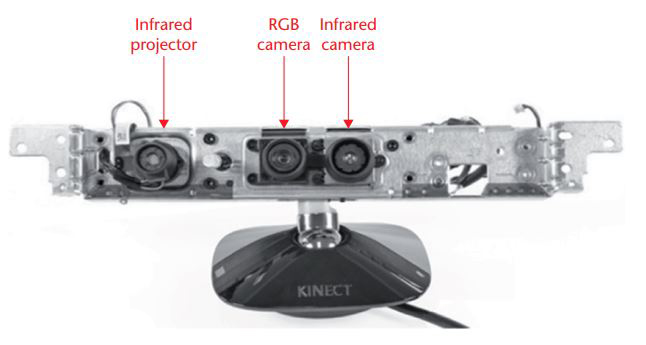
\includegraphics[width=\textwidth/2]{images/kinnect.JPG} 
\caption{Microsoft kinect camera system with the three used sensor units\cite{Zhang.2012}}
\end{wrapfigure}
The currently most used type of system for tracking hardware is a setup of a combination of RGB and infrared sensors for imaging an depth measurement.The first commercial system using this technology is the\textit{ Microsoft Kinect} system\cite{Zhang.2012}. The system uses a infrared projector and an infrared sensor to measure distances in the captured scene.
Newer systems that also incorporate depth sensing through infrared distance measurement are the \textit{Intel RealSense} system and the more consumer focused leap motion hand tracker. The\textit{ Leap Motion Controller} does not supply a separate RGB sensor and does therefore only provide depth measurement data within a specific range from the device\cite{Weichert.2013}.It combines two infrared cameras with three infrared emitter LED's, placing the system into the category if stereoscopic tracking systems.
\begin{figure}[H]
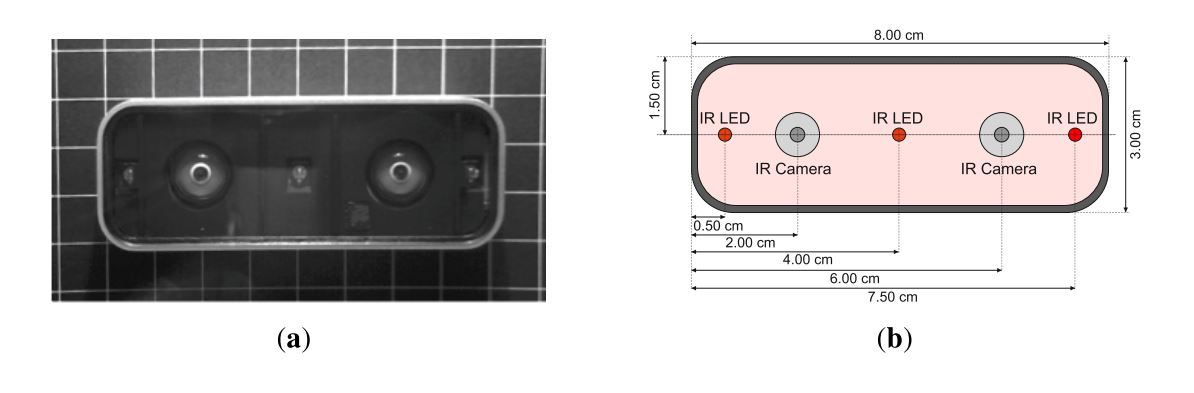
\includegraphics[width=\textwidth]{images/leapMotion.JPG}
\caption{Visualization of a (a) Real (using Infrared Imaging) and (b) Schematic View of Leap Motion Controller\cite{Weichert.2013}.}
\label{img:leapMotion} 
\end{figure}
The latest Product in this category are the \textit{Intel RealSense} camera systems\cite{IntelCorporation.2018}. The Intel systems, like the\textit{ Leap Motion Controller} utilize a stereoscopic infrared system setup, and can also provide RGB Sensor data, depending on the selected model.
\begin{figure}[H]
\centering
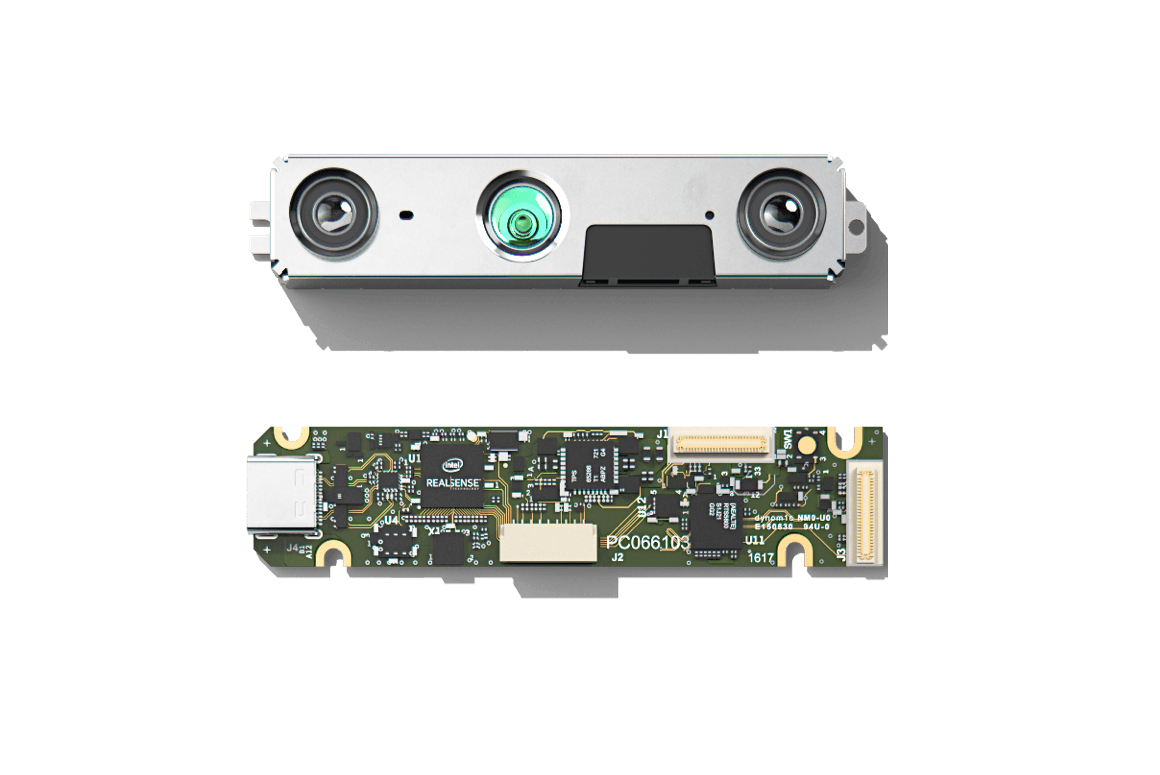
\includegraphics[width=0.6\textwidth]{images/RealSense.png}
\caption{Visualization of a \textit{Intel ReaslSense} depth module\cite{IntelCorporation.2018}}
\label{img:leapMotion} 
\end{figure}
The \textit{Kinect} can supply depth data at around 30 fps, it's modern  descendants from Intel can supply data at frame rates of up to 90 fps. The systems provide the convenience of not having to apply any form of distinguishable marking to the surface that has to be tracked. The downside of this feature is that the devices only supply SDKs for accessing the collected data from the device. The post processing of this data needs more sophisticated image analysis or neural network processing to figure out feature points of the tracked object from the supplied image data\cite{JamieShotton.2011,Oikonomidis.2011b}. Image analysis of large image can be costly for real time applications and the training of neural networks for the analysis can consume a lot of time and tweaking until the trained result fits the application.
\\An recent approach of combining RGB-D Data and the usage of CNNs (Convolutional Neural Networks) to estimate hand pose and render a correct digital representaion of the hand is shown in \cite{FranziskaMueller.2017}.
\\Their approach uses two subsequently applied CNNs to localize the hand and regress 3D joint locations. The first CNN estimates the 2D position of the hand center in the input. The combined information of the hand position together with the corresponding input depth value, is used to generate a normalized cropped image. this image is then fed into a second CNN to regress relative 3D hand joint
locations in real time. Pose estimation is furthermore refined by using a kinematic pose tracking energy toa chieve more accuracy, robustness and
temporal stability.
\\They also introduce a new photorealistic dataset that uses a merged reality
approach to capture and synthesize large amounts of annotated
data of natural hand interaction in cluttered scenes for CNN training data.







\newpage
%!TEX root = ../Masterthesis.tex
\chapter{Digital hand models}
After retrieving all needed data from the real world counterpart and calculation for pose estimation is finished, the returned solution has to be displayed in the digital world. Therefore a digital hand model is needed to represent the calulated data. Modern day computer animation techniques make it possible to create nearly photorealistic digital replicas of human skin wrapped onto anatomically precisely modeleld bodyparts. These highly complex modelsacquire a lot of calulation resources and are mostly not appropeiate for a realtime rendering approach.\\
When apdapting calcualtion data to digital hand models, those of lesser complexity are preffered, sacrificing the quality of the resulting output for speed and more fluent motion results.

\newpage
%!TEX root = ../Masterthesis.tex
\chapter{System prequisites}

Befor elaborating a final system conception, some perquisites have to be defined.

System components to be defined:
\begin{itemize}
 \item Display hardware
 \item Tracking Technology
 \item Tracking Hardware
 \item Data cleaning
 \item Image analysis
 \item Data cleaning
 \item Inverse kinameatics algorithm
 \item Hand model
 \end{itemize} 

 \section{Display}
 The first definition that has to be done is actually the last component of the processing chain. The final display hardware properties have to be defined initially as these are the determining factor for all other components. Since the goal of hand and object tracking is the most immersive when using a virtual reality headset rather than a normal display, these do not need to be taken into consideration.\\
Another device category which may be in the focus of interest are current mobile device platforms like \textit{Google cardboard} or the \textit{Samsung Gear} platform.In terms of creating an low cost consumer grade solution, these devices should be the first category to look at, as they are more widely available and do not need extra hardware except the smart-phone. Most modern devices have native support of WebGL in the browser, making it fairly easy to display VR content. They also come with the convenience of already having a set of integrated sensors for position an rotation integrated. The downside of this device class reveals when taking a look at the hardware specifications of these devices. Although the newest high tier consumer grade devices do have a good performance output for their size they are still no comparison for a desktop setup. Also these devices, as they are first of all mobile phones, show lacks for wire connections, making it necessary to mostly communicate over wireless protocols. This leads to a growth in infrastructure(server, wi-fi-hotspot, etc.) and every further node in the processing chain leads to a physical signal delay.\\
After these first preliminary steps, only pure VR-Headsets like the \textit{HTC Vive}\cite{HTC.2018}or \textit{Occulus Rift} \cite{OculusVR.2018}should be the main focus. These headsets also provide the capabilities of motion tracking while utilizing the processing capabilities of a dedicated GPU and high-power CPU capabilities of modern desktop computers. Furthermore, they provide a variety of connection ports for wired connections, eliminating the need for wireless transmissions. In terms of cost, these devices do lie on the more costly side as you need the headset itself and a hardware setup which is capable of providing the output frame rate needed. But with the latest generations of GPU's and CPU's, this category was opened towards the normal consumer.\\
The \textit{HTC Vive} as well as the \textit{Occulus Rift} are able to display 90 images per second on their displays with each having a resolution of 2160x1200 pixels, resulting in a little over full HD resolution per eye. The duration of one frame is therefore around 11 ms. This is the time frame in which the rest of the components can theoretically supply the image data, do the image analysis to retrieve the tracking data, recalculate the IK model, calculate the object position and render the whole scene before sending it to the headset to be displayed.
\section{Tracking technology}
Physical sensors placed on the hand tend to give more precise tracking results compared to optical methods. The cost for the data precision is that the sensors have to be mounted to the hand in some kind of fashion. Cables or fibers, depending on sensor type, can hinder the hand movement. Utilizing  a glove based system brings the downside of the " one size fits all" problem. Human hands can differ largely in size, therefore on glove will not be able to be used for a wide range of users. Furthermore cloth gloves tend to get dirty while usage and are therefore unsuitable in therms of hygiene.\\

Color markers can be utilized very easily. The simplest form could be colored electrical tape wrapped around the fingertips. These markers can be made disposable after usage. The size of the marker can be adapted to be large enough to realize a robust tracking while being small enough to not constrain hand movement. They also provide the possibility to perform a person specific calibration of the hand model in an initialization step.
The easiest way to detect color markers is to use an optical tracking system.
Monocular optical tracking system are relatively easy to set up as they only need one camera, the complexity in the later processing steps of evaluating the marker positions from  only a single frame rises drastically.\\
Stereoscopic system in comparison have a higher initial effort in setting up and calibrating the system, but the further processing steps are fairly easy. 

\section{Tracking Hardware}
 As explained int the previous chapters, the motion of the human hand can be complex and in some cases really fast. Therefore, the optical tracking hardware should ideally be able to record images with the same or higher frequency as the display medium that is to be used. Prosumer and professional grade cameras are theoretically able to produce these kind of Frame rates (60 fps and above), but most of the time store these high frame rate videos directly to a hard drive rather than broadcasting them somewhere as most of the current day devices are not able to display such high frame rates yet. Also the hardware that is needed to record such specific high frame rates is relatively expensive. Consumer grade cameras like the GoPro that are affordable, can record at a Frame rate of 120 fps but the live transmission of this material has a time lack of several frames.\\
\\When trying to utilize low cost hardware the limitation of recording and sending a video signal from a camera to a processing hardware will therefore be limited to 60fps. This process would also introduce further latency on the transport and would force a further reduction of frame rate to satisfy the time frame given by the display frame rate.
\\Another option that can be taken into consideration is to completely eliminate the need to transport the image data from camera to another device. This can be achieved when the camera and the computational hardware are located on the same hardware.\\The \textit{Raspberry Pi 3} microcomputer, which comes from the internet of things world provides this capability. It combines a for its size quite powerful computation capacity with an on-board hardware connector for a camera. The camera hardware is able to record in a FullHD resolution at 60fps and at lower resolutions up to 90fps. The camera module is directly connected on the the chipboard, providing direct access for further processing.\\
For a complete 3 dimension space tracking, a one camera setup is not sufficient as it lack the data for the depth position of the object. To get this data, further hardware is needed. One option would be the utilization of a time of flight based depth sensing system, but these system do come at a rather high entry level price.
\\Another option could be the tracking  pods that HTC offers as an expansion to it's vive system. These trackers could provide 3D positional data but with the downside of being relatively bulky. This would hinder the movement space of the hand and the tracker would have to be positioned on the arm as near as possible to the wrist. This would result in the position of only the wrist and not providing data on each individual finger of the hand. But as hindering as these trackers are on the hand, they could be easily used to provide tracking data for used objects. the tracker could be positioned onto the object where it does not hinder the usage. \\
Since the hardware setup of the Raspberry Pi with the camera is relatively easy and cost efficient, the usage of a second Raspberry Pi with a camera is good leverage point. The two cameras can be setup to create a stereoscopic camera setup which provides information about depth position through the disparity of the two camera images. 
Furthermore the image operations that need to be independently applied to each of the cameras frames can be done on the two separate device, eliminating the need for sending data traffic with image information through the network for post processing.
\\Downside of this method is that with all stereoscopic camera setups, the two cameras need to have some kind of frame synchronization to get the right two frames for evaluation.
\\The setup is not only meant for tracking the hand, but also for tracking objects in the tracking space, the system needs to be capable to do this task as well. Since the computational power of the raspberry is limited at some point, it is to be evaluated if a separate hardware component is needed for the object tracking or if the tracking can be integrated into the tracking procedure of the hand markers.\\% Another question that could be investigated would be, how important the depth position for the to be tracked object really is as they will not be floating in space while being tracked.
\section{Data cleaning}
Every system that deals with the computation of live data is suspect to data fluctuation in input and output values. It is also to be assumed that the system will not be able to achieve an ideal synchronization between the cameras. This will probably introduce a degradation of tracking performance which has to be handled. It has to be evaluated at which point a data cleaning will lead to the best end results.
\section{Image analysis}
The images recorded by the camera system need to be processed further down the line to get the positional data of selected hand features. The most common library to do such kinds of image processing is the \textit{OpenCV}\cite{OpenCVTeam.2018} library which is originally written in C and was ported into several other programming languages. It has build in features for camera calibration, color and object detection as well as several image optimization features that might be helpful for the processing.
\section{Inverse kinematics}
The inverse kinematics model is the second essential part of the setup after the tracking hardware. It receives the position data from the image post-processing and calculates the resulting current hand model position. The applied algorithm for the IK solution should be able to keep up with the data-flow from the tracking algorithm and should produce a fluid optical result on the display. As the calculation of the IK solution and the rendering of the scene with the models should be done on the same machine, computation power and memory consumption should be critical criteria. As the system will rely on optical tracking data, an algorithm that is capable of dealing with tracker occlusions and recovery from this data loss should be prioritized. 
\section{Hand model}
For evaluation purposes, a rather simple model form should be used for the representation of the tracked hand in the digital space. The outcome results for tracking accuracy, update speed and the resulting match of physical and digital position of the hand are of more relevance than a highly realistic hand model.
 
\newpage
%!TEX root = ../Masterthesis.tex
\chapter{System conception}
\section{Image Analysis with OpenCV 3 and Python on the Raspberry}
For the Image analysis part, openCV3 with it's python 3 bindingd is chosen. The OpenCV package needs to be downloaded and compiled onte each device be fore it can be used.

The python programm thath is used for tracking the specified color markers is comprised of the following components:
\begin{itemize}
\item Image acquisition from camera
\item Image conversion to HSV colorspace
\item Mask construction and Filtering
\item Contour finding an Position calculation
\item Sending of positional data via Network as UPD Package
\end{itemize}

\subsection{Image acquisition from camera}
As the computaion times for iamge filtering and mask generation may vary, it makes sense to seperate the image acquisition from the computation part. tehrefore the loading of the raw image data frame from the camera is outsourced into its own thread. Also this allows us to trigger the frame grabbing on both devices for synchronization. \todo {elaborate}.
\\The tread takes the fdata of the current image frame and hands it over to hte main thread, where the image processing is handeled.
\subsection{Image conversion to HSV colorspace}
The image data that is supplied by the camera comes in an RGB data format, which we could already use for the further calculation. It does though make more sense to convert the imput data into the HSV colorspace. Since we are not using high precision cameras, it is necessary to define a range of color values around the desired color which we want to track. The HSV colorspace is displayed as a cone, in comparison to the RGB colorspace, which is diplayed as a cube. The color values for the HSV space are all located on a cirle spanning form 0 to 360 degrees. The Hue value (H)corresponds to the angleon the cirlce, where $0\deg$ corresponds to a redish color, $120\deg$ lies inthe area of green and $240\deg$ and obove correspond to blue. The sturation value (s) coresponds to the amount of white the color contains  where 0 is pure white and 100 corresponds to the fully saturated color. For optimal results, only highly saturated colors should be used to ensure correct color detection. The last compoonent is the value component (V) which describes the intensity of the color. Alike the value settings for the saturation, value ranges of at leas 50 should be used for tracking precision.
//
For tracking the five fingers of the hand we need five distinguishable colors. Here the primary colors red, green and blue will be the choice for the first three colors. The other two selcted colors \todo {check test results} are orange and yellow. To be able to clearly ditinguis these colors in the video frame, a constant and homogenous lighting is needed as well as a color themeprature of the lighting that is in the neutral area to not change the color of the markers.
\\the color conversion from the input RGB values to the desired HSV colorspace is done as follows:
\begin{equation}
\begin{split}
hsv_{low}=(hue_{targetcolor}-sensitivity,100,100)\\
hsv_{up}=(hue_{targetcolor}-sensitivity,100,100)\\
\end{split}
\end{equation}
\subsection{Mask construction and Filtering}
\todo {orig image and mask images for display}
These values are the used as the parameters for a mask generation which generates a binary mask for the current frame where all pixels whose values lie outside of the specified range are set to zero (black) and the remaining are set to 255 (white).For these masks to work properly, any other larger objects thath might contain similar colors should be removed from the scene to eliminate worng tracking data. As all digital cameras tend to have signal noise in the sensor data , high frequenc  noise in the color channels will be present. This noise needs to be filtered out before any further computaion on the image data can be done.\\
The first step in this progress is to use a gaussian filter to blurr the mask. After this step an erosion and a dilation is applied to the image tho further eliminate unwanted noise.\todo {elaborate}
\subsection{Contour finding an Position calculation}
With the cleaned mask we can continue and search for the white areas in the mask which might represent our target. Under the assumption thath we have removed all other parasitic objects from the image, the marker should be the largest area of positive pixels in the mask frame. Therefore only the largest area found in the search is taken as the desirted tracking marker. For the selected area, a fitting bounding box is calculated and the center of this box is used as the posiitonal parameter of the tracking marker.
\subsection{Sending of positional data via network as UPD package}
The resulting data is then handed over to a seperate thread running a UDP server which sends the positional data to the parent device where the stereoscopic calulations as well as the hand model and rendering is done

\section{Technical conception}
\begin{figure}[H]
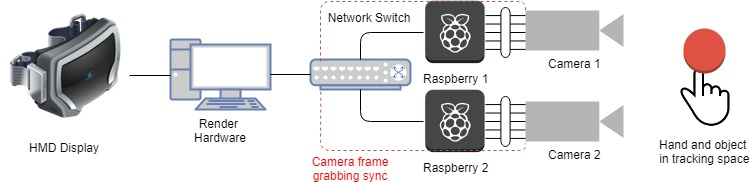
\includegraphics[width=\textwidth]{images/technical_setup.jpg}
\caption{Technical conseptiopn of the single hardware parts}
\label{technical-copnception}
\end{figure} 
The technical setup of the whole system is relatively simple. Instead of using one large dimmensioned Unit which takes care of all calculations, the image processing steps that have to be done on both stereo images anywy are outsourced onto the Raspberry Pis. As already mentioed in the conception Phase, the image processing dircetly on the rapspberry also reduces latency which would occur when sending image data over network channels to the main unit.\\
The two \textbf{Raspberry Pi 3 Model B}, which are used as the controllers for the\textbf{Raspberry Pi Camera V2} are connected via network cable to a network switch. A connection over wireless Network would be possible with the onboard capabilites of the  Pi's, but here we might encounter latency problems and/or signal interference with other exisitng networks. Therefor a cable connection is the safer solution.
The switch also connects to the "Master" PC to which the "Slave" Pi's communicate their data. The Master also takes care of the stereoscopic calculations,as it is dimensioned with far more computing power than the slaves.The 2D positional data from the slaves and dthe calculaton results from the stereo image disparity is fed into the hand Model running on the "Master". The model solutionis then applied to the digital hand model and rendered to the HMD.

 





\newpage
%!TEX root = ../Masterthesis.tex
\chapter{System Evaluation}
\begin{figure}[H]
\centering
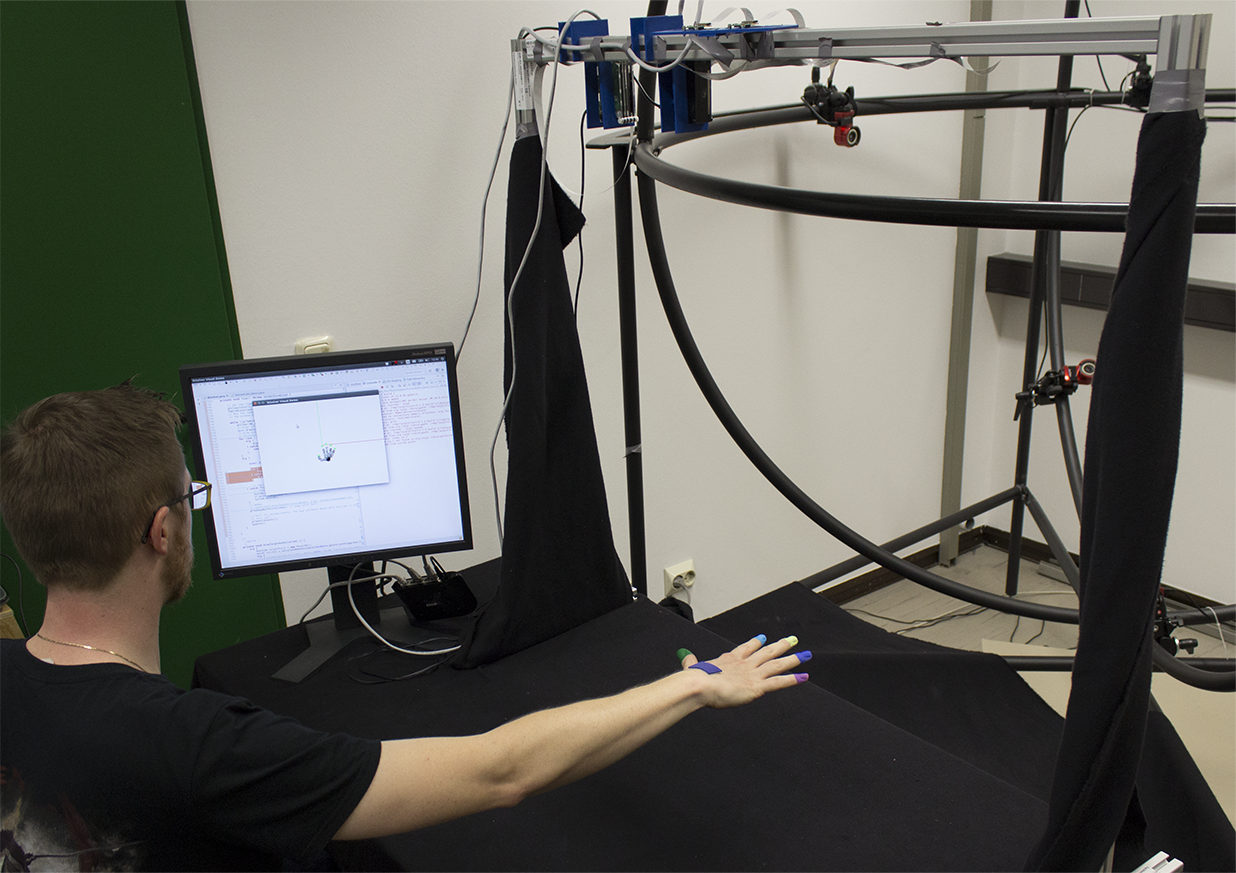
\includegraphics[width=0.9\textwidth]{images/complete_setup.png}
\caption{Final system setup with cameras on construction profile, color markers and visualization.}
\label{img:complete_setup} 
\end{figure}
\section{Camera hardware and control}
The Raspberry Pi image processing of the camera frames can be a significant bottleneck for the system. "Real-time" evaluation demands the processing time of a frame to be in the range of the time of the camera FPS to utilize all available frames. With the current system setup limited to 30 fps by the camera framework, the image processing has to be done in about $1/30s$ or 33 ms to achieve "real-time" processing. Professional stereoscopic setups use cameras with global shutters and a synchronization signal. This enables a sub-frame synchronization of the two camera systems. The cameras used in the prototype setup use a rolling shutter instead. Furthermore, these cameras are designed to be of easy use for the normal consumer, therefore their design does not incorporate a synchronization feature. To achieve a form of hardware synchronization, a large amount of reverse engineering would be needed as the electrical drawings as well as the controlling software are closed source. The multi-layered circuit board of the camera would also complicate the reverse engineering step.  For these reasons, attempting the synchronization of the data further down the processing pipeline was more reasonable.
\\To synchronize the  frame reading of both cameras, the system boots up to the point where all needed components are initialized. At this point, the program waits for a start message from the "Master" system via \textit{UDP}. The "Master" system send the start message at the end of its initialization phase via a \textit{UDP} broadcast.This ensures that both Raspberry's get the message at the same time.
In normal usage mode, the camera uses automatic modes for it's parameter setup. This continuous measuring mode produced fluctuation in image brightness and color saturation. To eliminate this problem, all automatic modes were turned off in the camera initialization phase. Fixed values are loaded from a \textit{JSON} file instead. To get the values for the \textit{JSON} file, a calibration step was implemented. This calibration step enables the user to preview and manipulate the following values for the camera:
\begin{itemize}
\item Saturation
\item Brightness
\item Gain
\item Exposure time
\item Contrast
\item White balance values for blue and red channel
\end{itemize}
\begin{figure}[H]
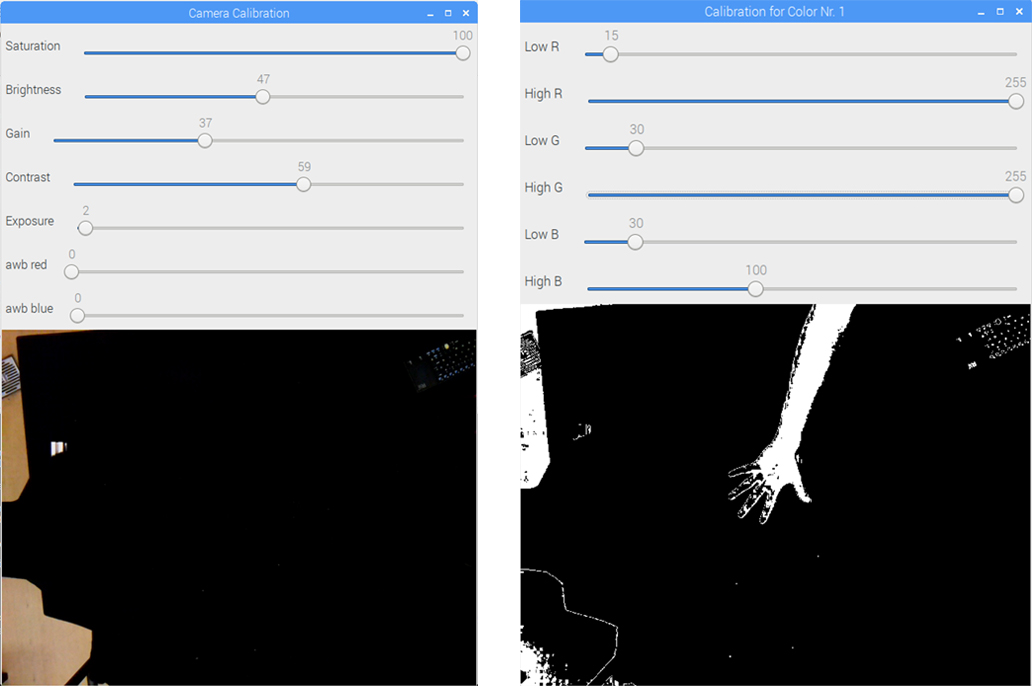
\includegraphics[width=\textwidth]{images/calib_windows.jpg}
\caption{Camera and color calibration utility window}
\label{fig:calibration_windows} 
\end{figure}
The user-set calibration values can be written into a new \textit{JSON} file. They are directly loaded into the program after calibration is finished. Control over these parameters showed to be crucial for achieving a constant color separation. The threshold values for the color tracking also needed to be initially calibrated. These values are dependent on the lighting situation and any change results in the need for re-calibration. To simplify this calibration, a calibration functionality in line with the camera calibration was implemented. The implemented feature provides the user with a preview of the resulting thresholded black and white image with applied camera settings. Range sliders for lower and upper boundaries for the three RGB components make it fairly easy to adjust and view thresholding results in "real-time". The calibration values can also be stored into a \textit{JSON} file. This file can then be read out on following program start-ups.
\section{Image processing performance}
The first prototype implementation with \textit{OpenCV} in \textit{Python} showed, that a speed of 33 ms was achievable when only tracking one color. The implementation reached around 30 - 40 ms processing time when scanning whole images. An implementation of an \textit{"Region of interest"} feature reduced the processing time to around 30 ms for a single color. The downside of the implementation was revealed when implementing the other 4 colors needed to do a full five finger tracking. This approach ramped-up processing time to around 100 ms per frame, making this solution run at 10 FPS.\\\\ 
The sequential algorithm also showed another design flaw. When not utilizing the ROI approach, the algorithm would scan the whole grabbed camera frame for each color to create the corresponding threshold map. The \textit{OpenCV} color threshold methods are designed to only search for one color threshold at the time. They therefore need this procedure. One solution option is the already mentioned data reduction through ROI usage. This solution could furthermore benefit from a multi-threaded implementation. The original image data is only read. Parallel memory readout is not a problem and the generated mask can be saved separately.\\
\\Another approach which could help speed up the process is implementing an own method for thresholding the grabbed frame. This would result in the possibility to do all the needed color thresholds in one image loop. With this solution, the overhead would be reduced by 4 image iterations. The thresholding operations would stay the same as these still have to be run on each pixel. The output of this method would then return the 5 needed threshold mask for further processing.\\\\
A second performance issue that arose from the first prototype was that the input camera frames are RGB coded. For better options of color separations, the image was initially intended to be converted into HSV colorspace. This operation turned out to be second longest operation after frame grabbing. \\Testing of the cameras indicated that the color separation in the original RGB images of the cameras is good enough for the used test colors. This caused this step to be omitted and shaved off several milliseconds of processing time.
The rest of the processing steps are performed in the sub-millisecond range and are therefore not as valuable for performance optimization.
\\The results from this prototype indicated, that the \textit{OpenCV-Python} combination is not suitable for reaching the 30 ms target time. The OpenCV library used by python is actually just the ported version of the C code library with bindings for python. As \textit{C} and \textit{C++} are more hardware near and therefore more performant, a second prototype implementation was done in \textit{C++}.
\\\\The recreated workflow of the Python code in\textit{ C++} initially showed similar performance measurements when using a sequential approach. This was to be expected, as it is the same code the Python bindings are using. Further investigation into code timings showed, that another bottleneck was the image optimization feature which applied erosion and dilation operations to remove high frequency noise in the image. This operation brought the time up to 100 ms processing time when processing the whole frame area.This  makes the implementation not usable for "real-time" application. Removing this feature when scanning full frames resulted in a major speed up of processing time. \\
The implementation of a thread pool, which handles all the color detection jobs, brought down the calculation time for 5 colors to around 120-140 ms. Although these times are still not usable for real time, it brought a significant performance boost. Figure \ref{c++ work flow map} shows the initial structure design of the program with a camera frame buffer and the thread pool approach. The cyclic buffer was intended to hold images frames for readout where camera frame rates are much higher than the achieved processing rates of the source code.Since the frame-rates of the current setup are slower than the time spend on processing, the image-buffer for the camera is not needed. The feature is left in the code but is not actively used at the moment.\\
\\\\Since the thread pool approach still took too long, a test with lower resolution than 640x480 was done and showed that the calculation time can be reduced. This indicated that the ROI idea would be feasible for further performance optimization. A test at a frame resolution of 320x240 pixels reduced the processing time for all five colors to below 10 ms.\\Utilization of the knowledge from these tests led to the implementation of the aforementioned\textit{ "Region of interest"} feature.
The first frame is analyzed as a whole frame, optimally resulting in the detection of a marker. As the marker detection creates a rectangle around the tracked area, we already have the coordinates for the ROI and only have to add an offset to this area.
\\The value of the ROI offset has to be set high enough to ensure that in the following frame, the tracking marker is still contained. It also has to be ensured, that the generated ROI is clamped to the frame dimensions. If not doing so, parts of the readout are can be located outside of the image plane, causing readout errors when used for the subsequent frame.
\\The following frames will then be processed with the input of the ROI, selecting only the defined section of the image and updating the ROI with the new data for that frame. The \textit{C++} implementation brought down the processing time as assumed. This made it possible to apply the image improvement operations that were left out on the python implementation.
\\Performance measurement for tracking consistency with stationary color trackers was performed for a time period of 10.000 frames to get qualitative results. 
A sequential implementation with the usage of the ROI and image optimization was used for better analysis options and showed an average processing time of 46 ms with a standard deviation of ~11 ms.\\
\begin{figure}[H]
\centering
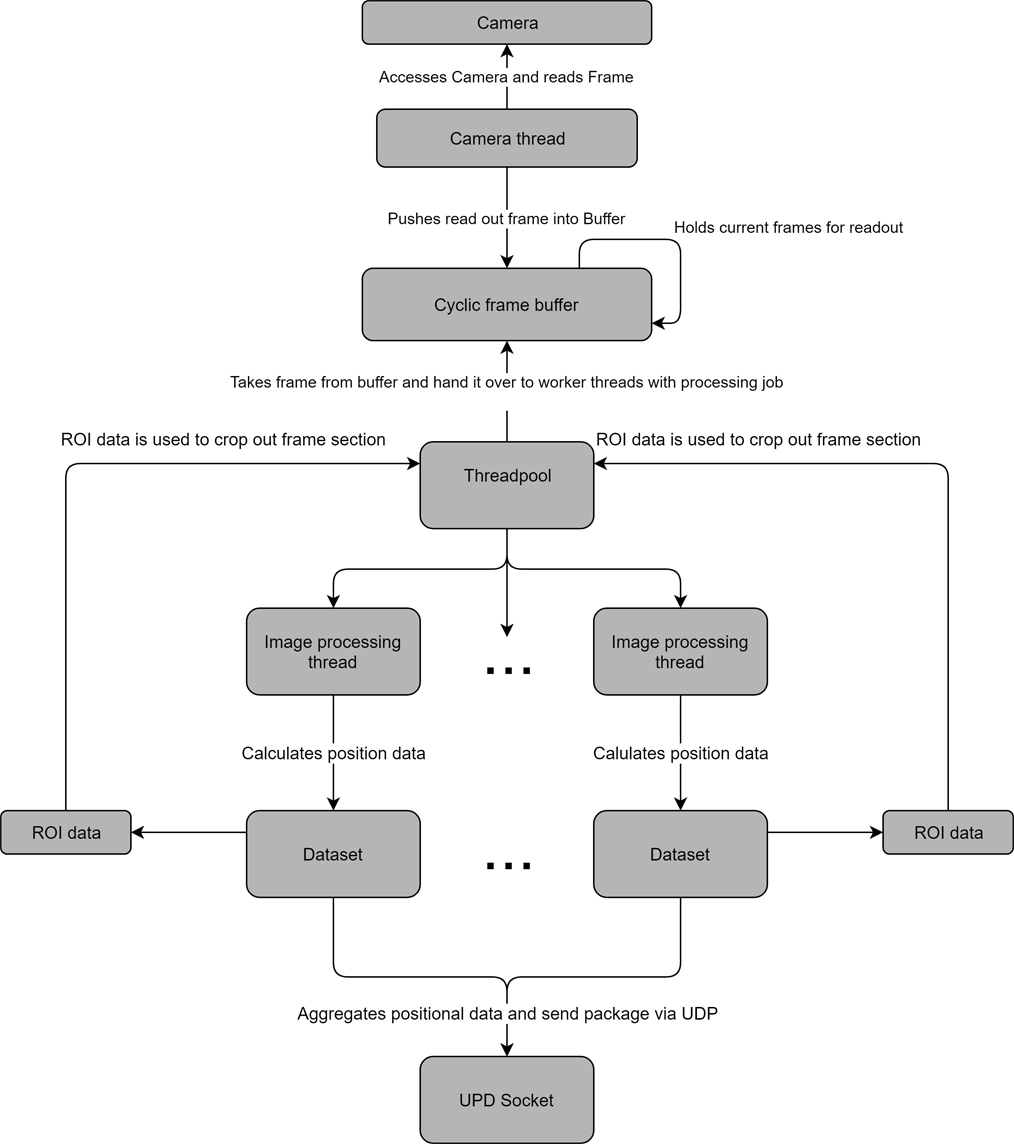
\includegraphics[width=\textwidth]{images/pi_workflow_500.jpg}
\caption{Intended work-flow of the C++ implementation with thread pool solution and ROI for high frame-rate solutions}
\label{c++ work flow map} 
\end{figure}

Further analysis showed that the high standard deviation came from peaks in performance times that took up to 400 ms when loosing tracking.\\ Filtering all values over 50 ms out from the data set showed that only $1\%$ ($\sim 1000$ out of $10.000$ frames) of the recorded processing times were lying outside of this time frame. Filtering out these values form the data set and recalculation dropped the average processing time down 3 ms to around 43 ms. The standard deviation was dropped drastically from its previous 11 ms to around $1.6$ ms. This shows that a filtering of processing times on the Raspberry could lead to a more consistent frame processing time. To do so, after every processing cycle the time should be checked. If it is over the defined time limit, no data should be sent.\\
Since this performance measurement does not give deeper insights on which part of the process consumes large amounts of processing time, the same measurement was done with a finer time tracking on the single parts of the processing pipeline.
\begin{table}[H]
\centering
\caption{Measurement results for sequential processing timing}
\label{tbl:sequential_performance_values}
\begin{tabular}{|c|c|c|c|c|c|}
\hline
\begin{tabular}[c]{@{}c@{}}Time \\ in ms\end{tabular} & \begin{tabular}[c]{@{}c@{}}Image \\ retrieval\end{tabular} & \begin{tabular}[c]{@{}c@{}}Stereo \\ rectification\end{tabular} & \begin{tabular}[c]{@{}c@{}}Color detection\\ (6 colors)\end{tabular} & \begin{tabular}[c]{@{}c@{}}UDP \\ sending\end{tabular} & \begin{tabular}[c]{@{}c@{}}Summed \\ time\end{tabular} \\ \hline
Average                                               & 0.92                                                  & 31.39                                                       & 14.55                                                             & 0.12                                                & 46.97 \\ \hline
Std.Deviation                                        & 0.17 & 7.19 & 5.06 & 0.06                                                & 10.77                                               \\ \hline
\end{tabular}
\end{table}
Table \ref{tbl:sequential_performance_values} highlights the performance bottlenecks of the system. Image retrieval from the camera as well as the time to process and send the data results via UDP are in the sub millisecond range. Therefore they impose no significant delay. Without these two steps, the remaining 96\% of the processing time is taken up by the image stereo rectification and the color tracking. When comparing these two, the far larger time consuming part is taken up by the stereo rectification part with nearly two thirds of the processing time.\\
The use of the stereo rectification in the system was done to ensure that the two used images have an aligned horizontal orientation. This is needed for camera pairs that are not aligned horizontally and/or parallel. Since the camera mounting ensures that the cameras are aligned parallel and at the same horizontal height, the rectification step can be omitted for performance reasons. It cuts down 67\% of the processing time of the system. As the stereo calculation does not use the vertical position difference for calculations, the possible resulting differences can be dealt with via filtering on the receiver side.
A solution for the color tracking time improvement was already described before. Utilizing a multi-threaded approach could lead to further reduction of the processing time.\\\\ A comparison between the before mentioned sequential algorithm with ROI and a multi-threaded implementation with ROI was tested as well. The multi-threaded implementation was designed to run the same processing stack as one loop of the sequential approach on each thread. Measurements over 10.000 frames for stationary as well as moving targets were made. One camera was run with the sequential implementation, while the second one ran the multi-threading approach. Thereby it is ensured that both cameras have the same measurement conditions.\\
The comparison of the measurements showed that in the current implementation state, the multi-threaded approach seems to have a much longer processing time. 
\begin{table}[h]
\centering
\caption{Measurement values of implementation comparison}
\label{tbl:implementaion_comparison}
\begin{tabular}{|l|l|l|}
\hline
Measurement            & Average (ms) & Std. Dev (ms) \\ \hline
Single-thread static  & 16.96        & 4.03          \\ \hline
Multi-thread static   & 32.09        & 10.64         \\ \hline
Single-thread dynamic & 19.41        & 22.44         \\ \hline
Multi-thread dynamic  & 35.80        & 22.88         \\ \hline
\end{tabular}
\end{table}
Table \ref{tbl:implementaion_comparison} shows that the measured time are roughly twice as long as the code running on a single thread. This behavior may result from an design or implementation fault in the multi-thread code and should be evaluated in future works to improve processing performance of the system. For the current state of the prototype, the single-threaded implementation with it's average processing time of around 19 ms is sufficient.
\newpage
\subsection{Color accuracy and ROI size}
As already mentioned in the conceptional phase, the lighting of the tracking area is a major factor. Variations of lighting intensity and color temperature cause the color of the trackers to shift their color. This can cause a fluctuation in the calculated tracker positions, as the defined color threshold ranges are kept as small as possible. This was done to achieve a clean separation of the tracker colors and reduce unwanted noise. \\\\
System testing with the 5 different colored shrink tubing markers proved, that the color tracking for colors outside of the color range of the human skin tones (green,blue) is rather unproblematic. The color markers falling into the colorspace of possible light reflection from skin may cause problems, depending on the lighting situation of the setup.
\begin{figure}[H]
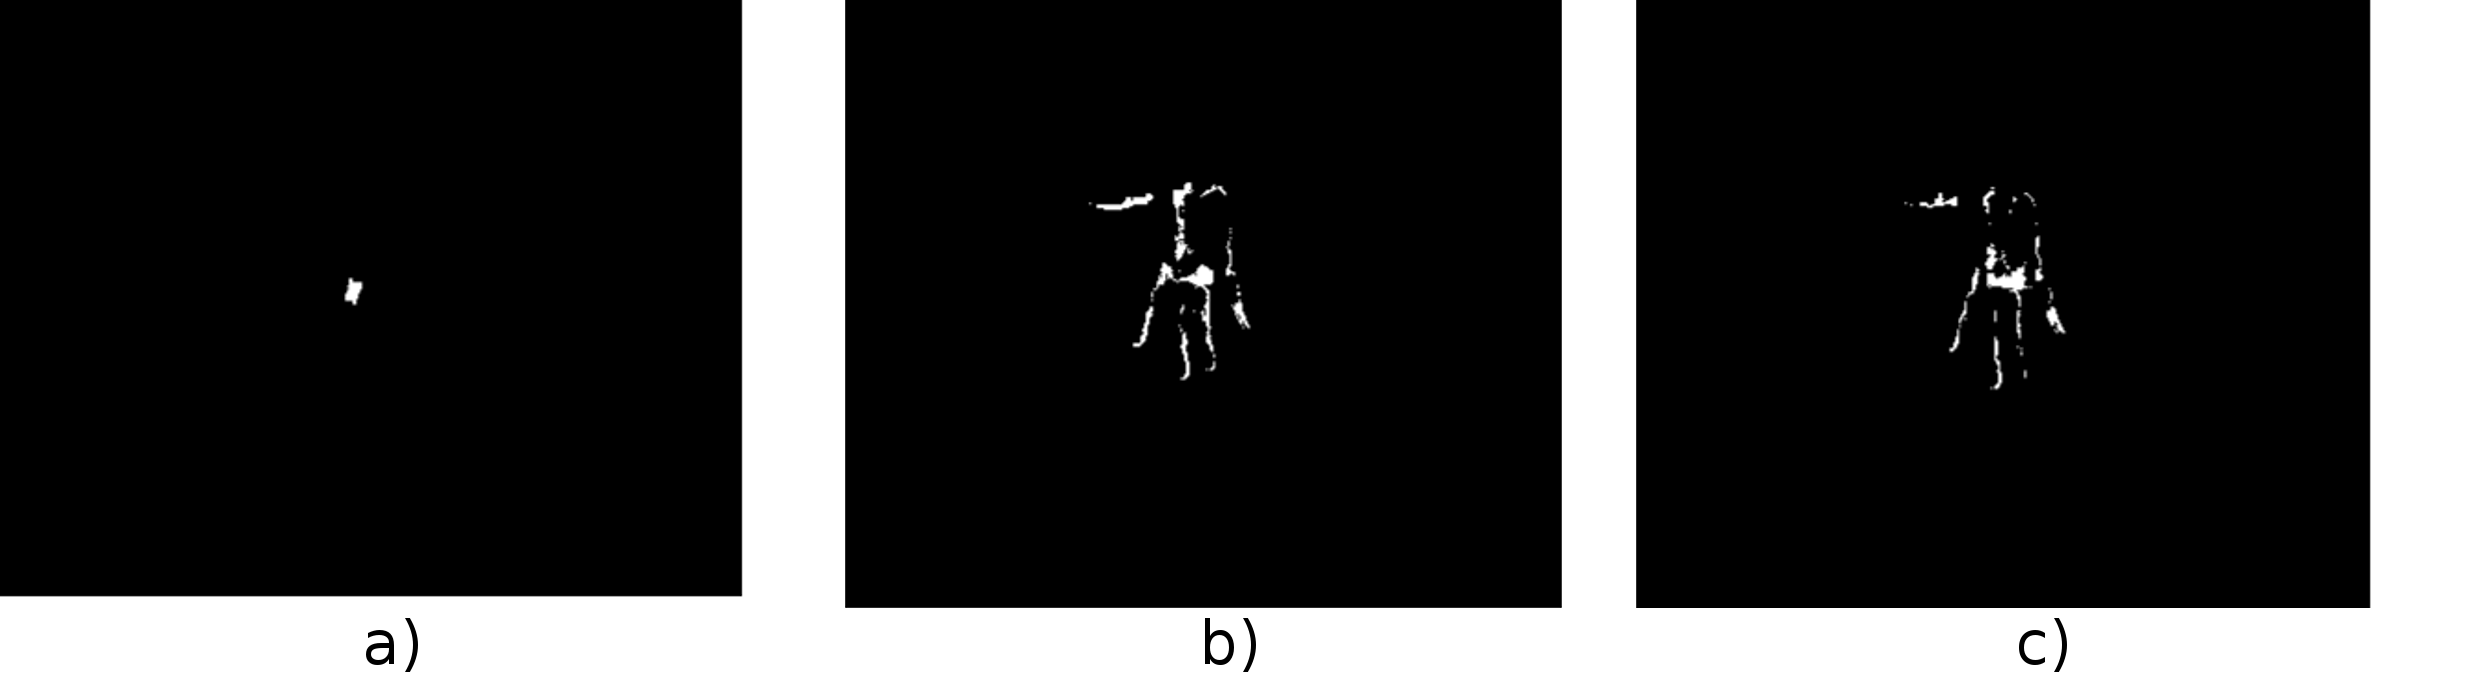
\includegraphics[width=\textwidth]{images/color_tracking_probs.png}
\caption{Images showing reflection problems with  orange color thresholding. a) Correct threshold with only the marker being thresholded b-c) Depending on the rotation of the hand, skin reflection color falls into tracking threshold.}
\label{img:Color_reflecton_problems} 
\end{figure}
Figure \ref{img:Color_reflecton_problems} displays such a case where depending on the orientation of the hand, reflection from the scenery lighting can fall into the color tone space of the tracked marker. This can cause large parts of the hand to light up in the image. Since the calculation of the tracking marker position relies on finding the largest closed "white" area in the thresholded image, this can cause a "jumping" of the calculated position. 
\\\\The first solution for this problem is to narrow down the color threshold spans. By doing so, one can ensure that only the wanted colors are tracked. This method does have a downside effect. When the markers are moved in the tracking space, light variations and shadowing will cause the colors to shift their appearance slightly. With broader threshold ranges, this does not seem to be a large problem as these changes still lie inside the ranges. Narrowed down color ranges might not include these color variations. It could also create cavities in the thresholded image.\\ The applied morphological operations on the image can fix these problems up to a certain point, depending on filter kernel size, but for larger areas this could vary position tracking results.\\\\The implemented ROI feature speed up the whole system calculations once the colors are found. Before this point, the system scans whole frames to find colors, which takes more time than the much smaller ROI regions.
Empirical evaluations showed, that for the used tracking space, a ROI region size offset of 40 px in x and y directions produces the best results in terms of consistency. Smaller region offsets caused the system to use tracking for faster hand motion, which causes system slow down until the tracking has recovered. Larger ROI's showed to produce more consistent tracking results at the cost of higher calculation time.
\subsection{Finger markers}
\begin{wrapfigure}[19]{r}{0.3\textwidth} 
\centering
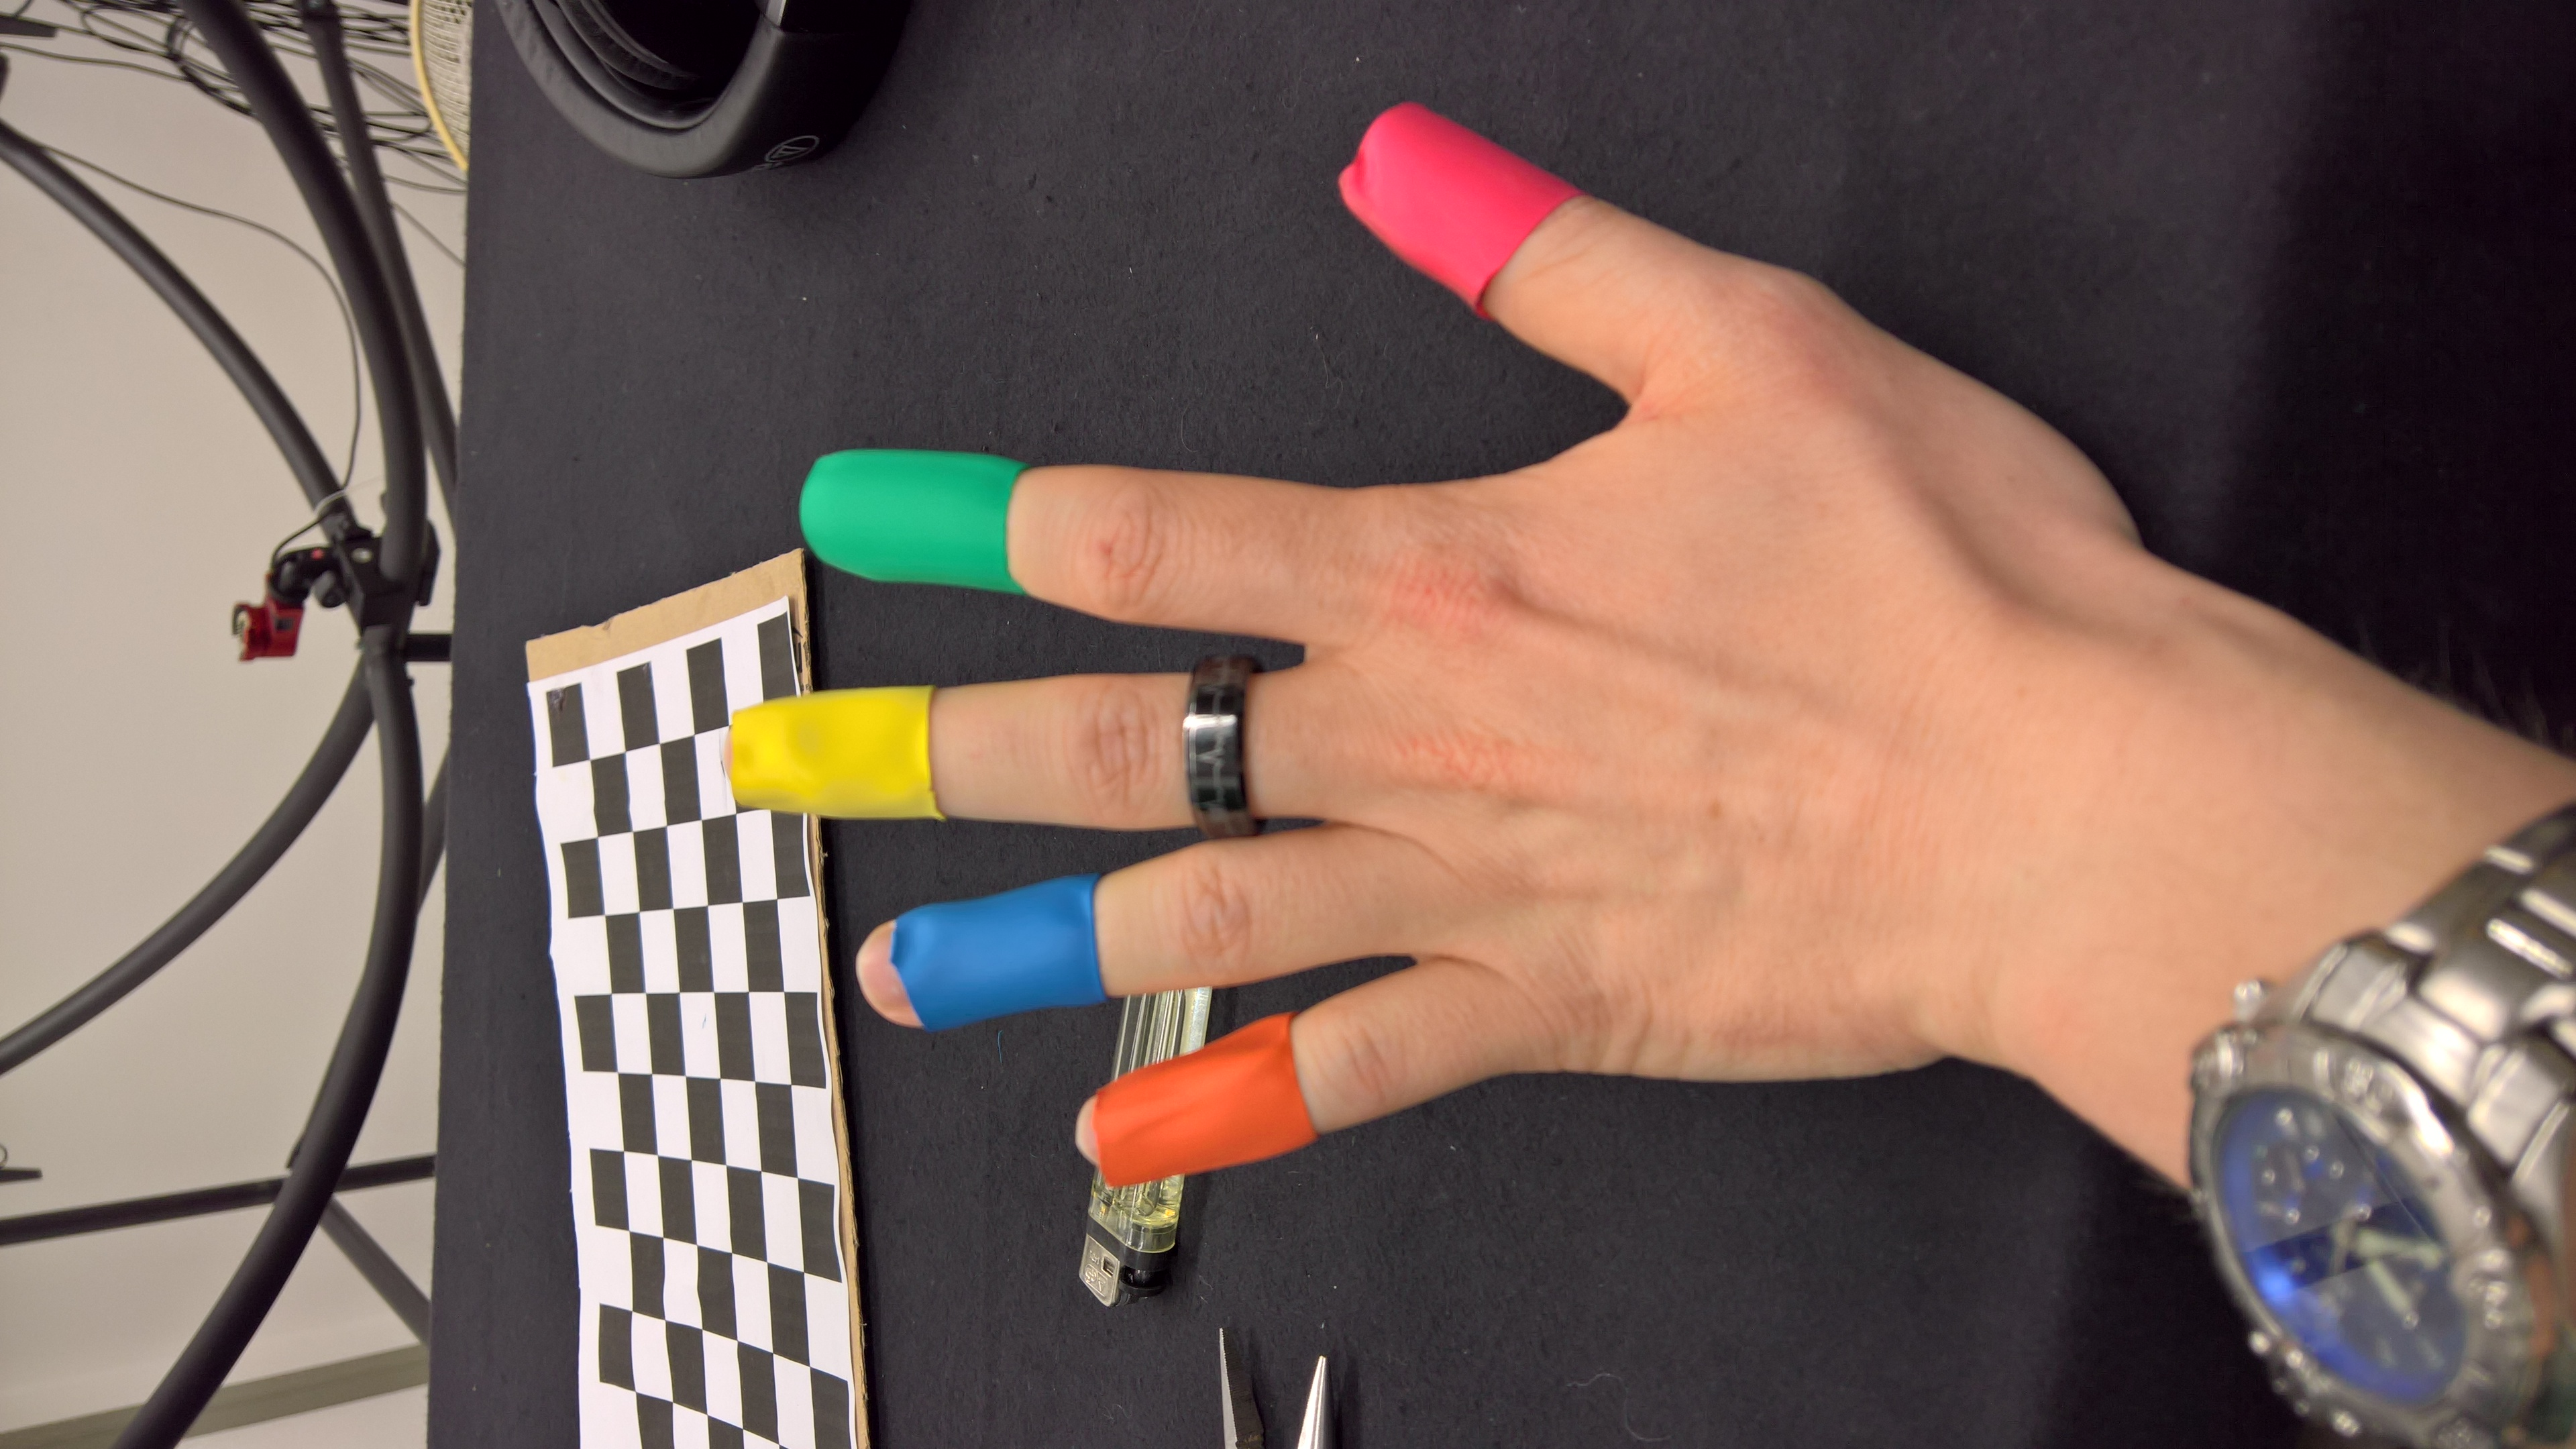
\includegraphics[width=0.5\textwidth,angle=-90]{images/color_markers_hand.jpg}
\caption{First set of shrink tube color markers }
\label{img:first_set_color_markers}
\end{wrapfigure}
The initial color marker size was selected to be relatively large, spanning most of the last segment size of each finger.
The used material of the colored shrink tubing was selected because it seemed to be relatively diffuse and therefore unsusceptible to errors resulting from the reflection of the scene lighting. The material turned out to be mostly diffuse reflecting, but depending on color and angle of light incidence, reflections in the color of the scene light did occur. A test-set of smaller markers was also evaluated, showing the same color reflection problems.\\The benefit of a smaller marker size would be much lower restriction of the finger movements and also unveiling the fingertips for better haptic interaction.
\\\\As both markers showed the above described problem of mixing marker area with possible skin reflections, an improvement to the markers was applied. At both ends of the larger markers, a piece of gray colored tape was applied to create an artificial border for the tracking algorithm.
\begin{figure}[H]
\centering
\includegraphics[width=0.5\textwidth]{images/small_and_improved_markers.jpg}
\caption{Improved larger and smaller set of shrink tube color markers }
\label{img:second_color_markers}
\end{figure}
The idea behind this solution was to create a fixed border between the color area of the tracker and the color area of the skin tones. The grey color of the border ensures that this area will not be tracked. The usage of black instead of gray would even furthermore ensure this. 
\\Since the threshold algorithm searches for the largest closed color area in the binary threshold image, this border should cause a separation of unwanted skin reflection area and actual tracker color area. The problem that the resulting color marker area might not be the largest area still persists after this improvement, but this case has to be handled separately.
\\\\Optical results showed that for the colors lying outside of the red to orange color spectrum that skin reflections produce, the artificial border stabilized the color detection.
\\The idea of using shrink tubing as marker material showed to be suitable except in the cases described above. One downside of the material is that the displayed colors are already the highest variety of available colors on the market. Other colors from the green and blue color areas like purple are simply not available or have to be ordered as a special request in larger amounts.
\\\\The original diameter is much larger than a human finger. The used shrink tube is able to be shrunken to one third of its size. The reason for this was to be able to adapt to the varying diameters of the human fingers. The shrinking procedure requires a constant amount of heat to be applied to the material to activate shrinking. The amount of heat that is needed surpasses the heat production of a standard hair dryer. The original application of shrink tubing is on heat resistant cables. The heat that needs to be applied can easily be more than 100 degree Celsius, which makes a direct application on the users hand highly insecure.
\\\\For the prototype, the shrink tube parts were shrunk with a standard cigarette lighter and continuously fitted onto the user finger until the desired form was reached. This method showed to  be sub-optimal, since the flame of the lighter produces only a punctual heat source. This caused uneven shrinkage of the heated parts. This can lead to cavities or bumps in the material. It  also changes the reflection properties at these points. A regulated heat gun would probably generate better results.
\\To get smoother shrinking results, parts of PVC tubing with the correct diameter could be used as dummy parts for the main part of the shrinking.\\
\\Another approach that was tested was the usage of matte acrylic paint to cover parts of the finger. The paint comes with the benefit of being easily to apply to the finger. Acrylic paint is available in much more color variations than the shrink tube. The finger coating is dry in under a minute after application. Adaption for finger size is automatically included in the application process. If the tracking system does not need to evaluate for hand rotation, i.e. the working principle is a top on view, a nail polish style application of the color on the fingernail can be sufficient for the tracking system. The thumb needs to be treated separately, as it has more rotation capabilities than the other fingers. It should be marked completely on all sides to achieve a constant tracking. If hand rotation is tracked, the other fingers should be completely marked as well.
\begin{figure}[H]
\centering
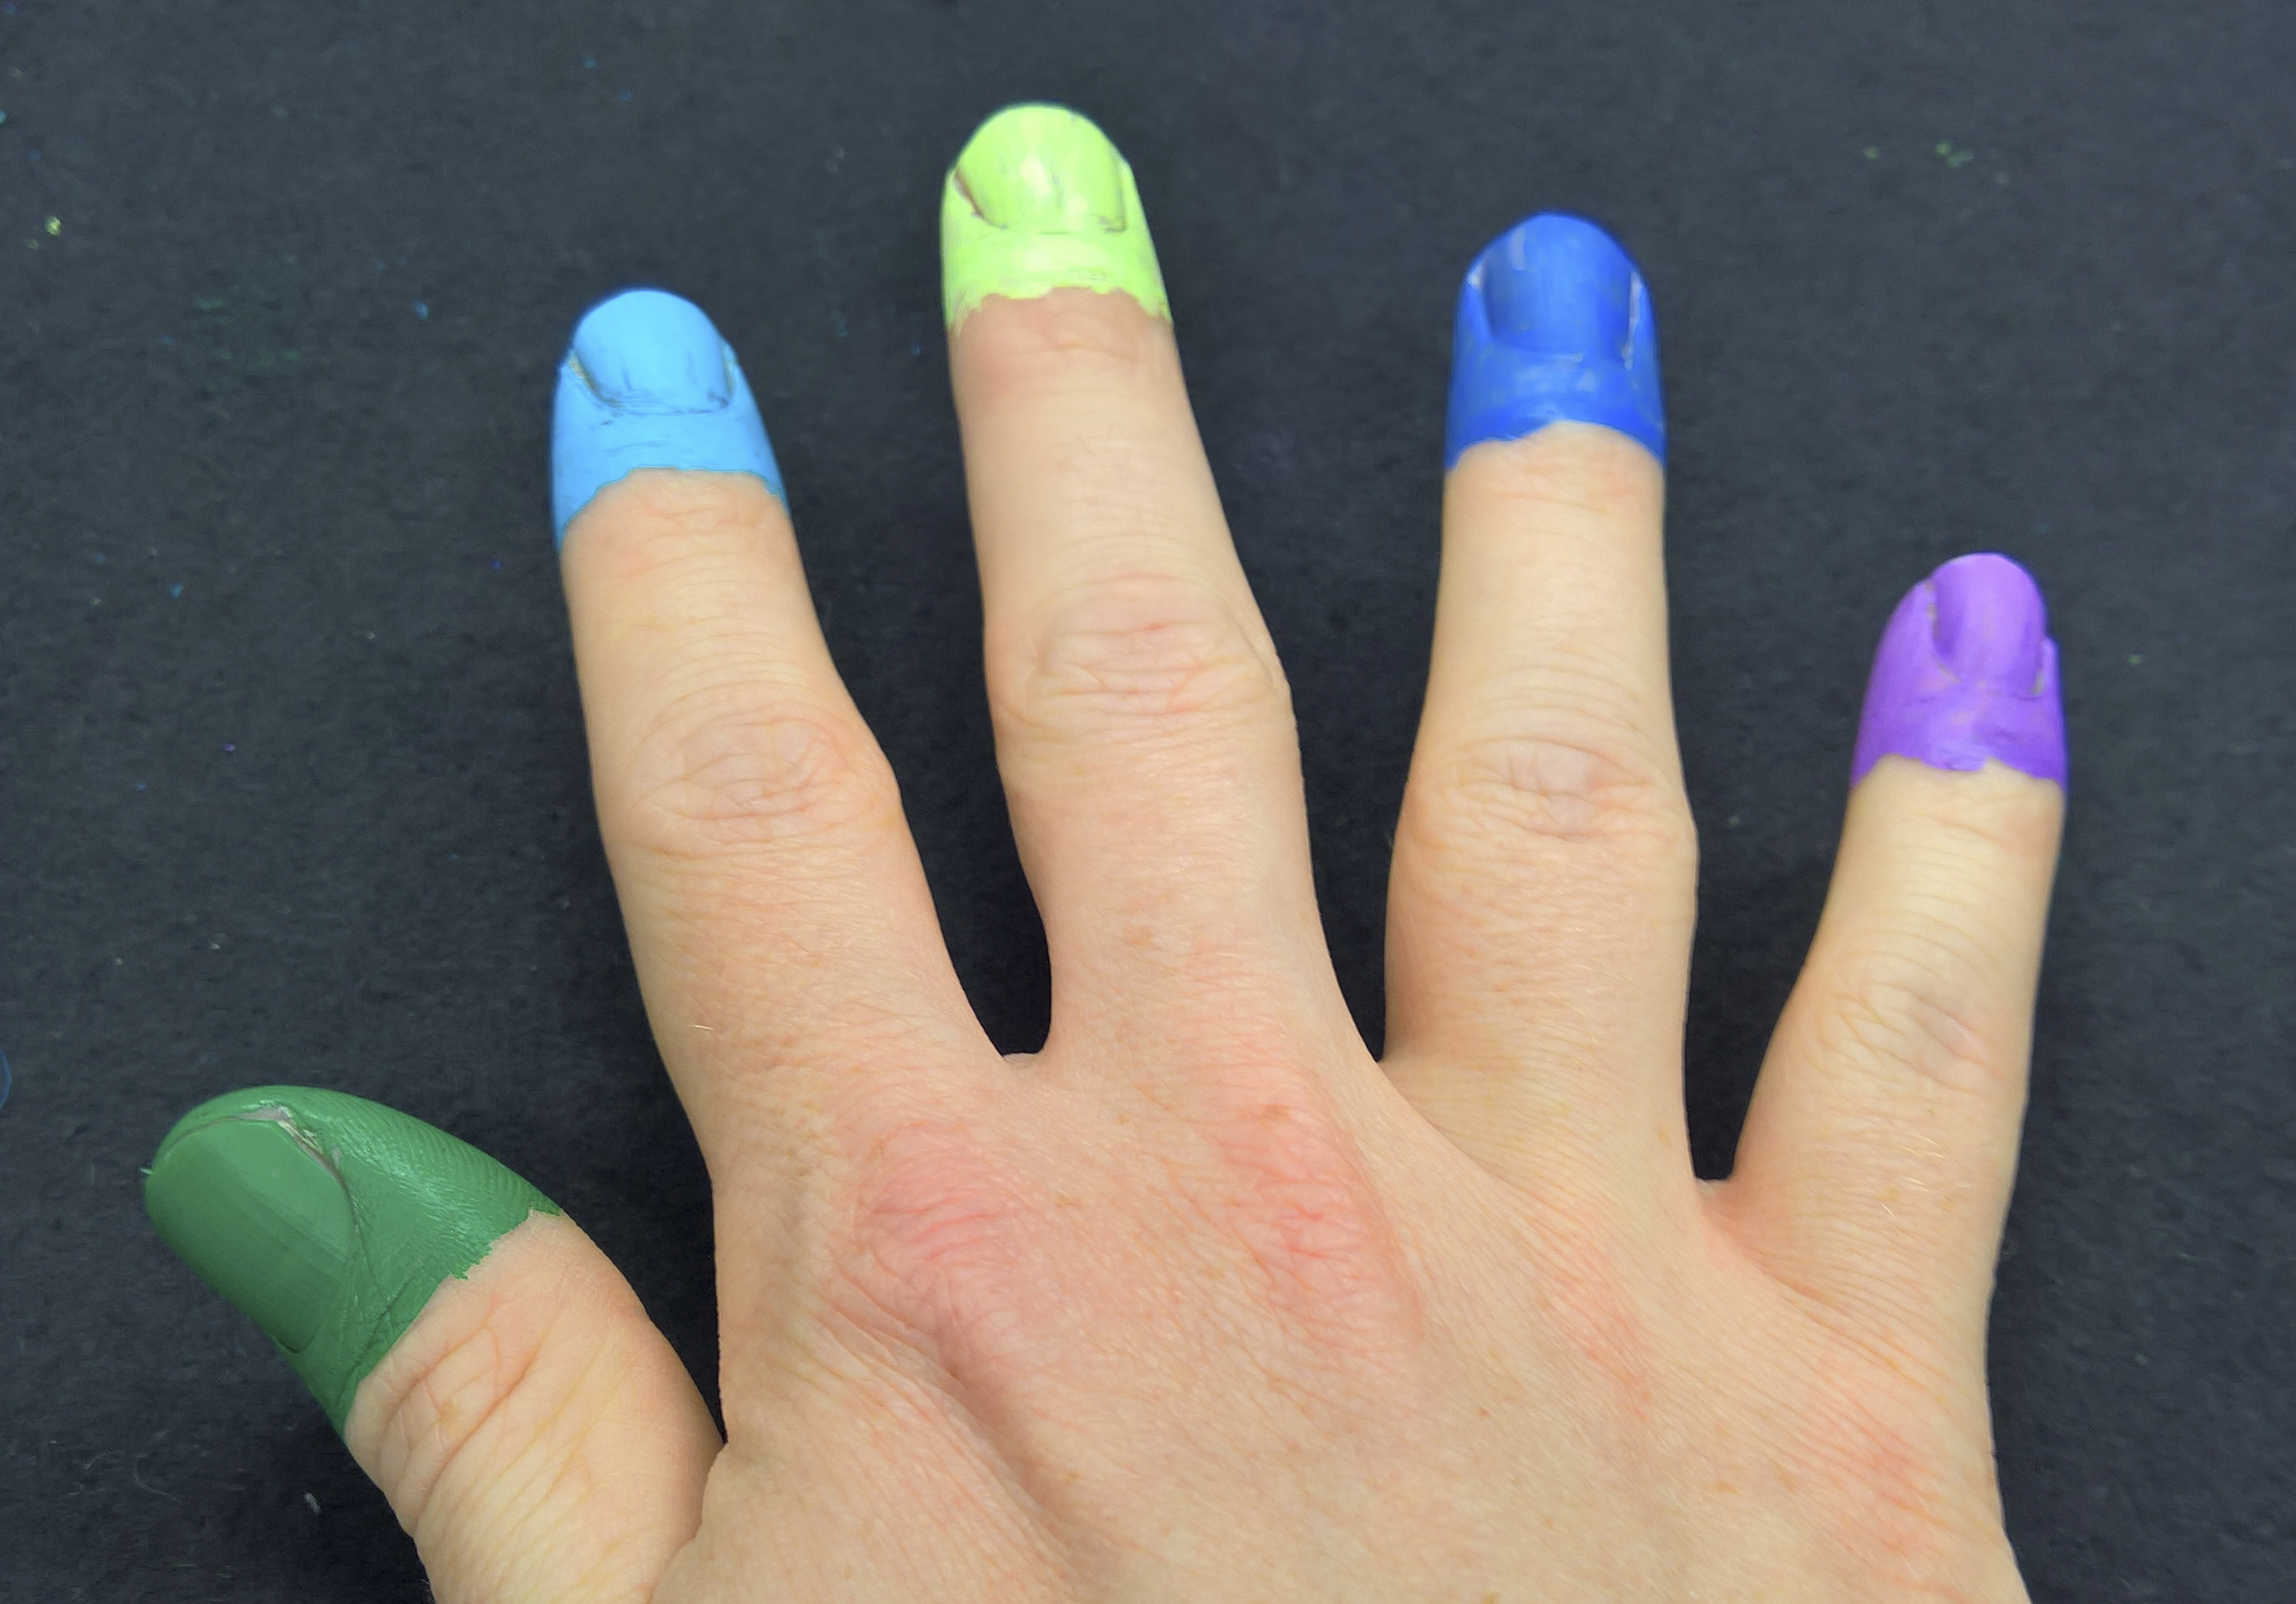
\includegraphics[width=0.5\textwidth]{images/final_finger_markers.jpg}
\caption{Finger marked with suitable acrylic colors}
\label{img:final_markers}
\end{figure}
\newpage As the final marker material, a mixture of blue and green color tones together with red tones in the purple and magenta section based on the acrylic color was chosen.
\begin{figure}[H]
\centering
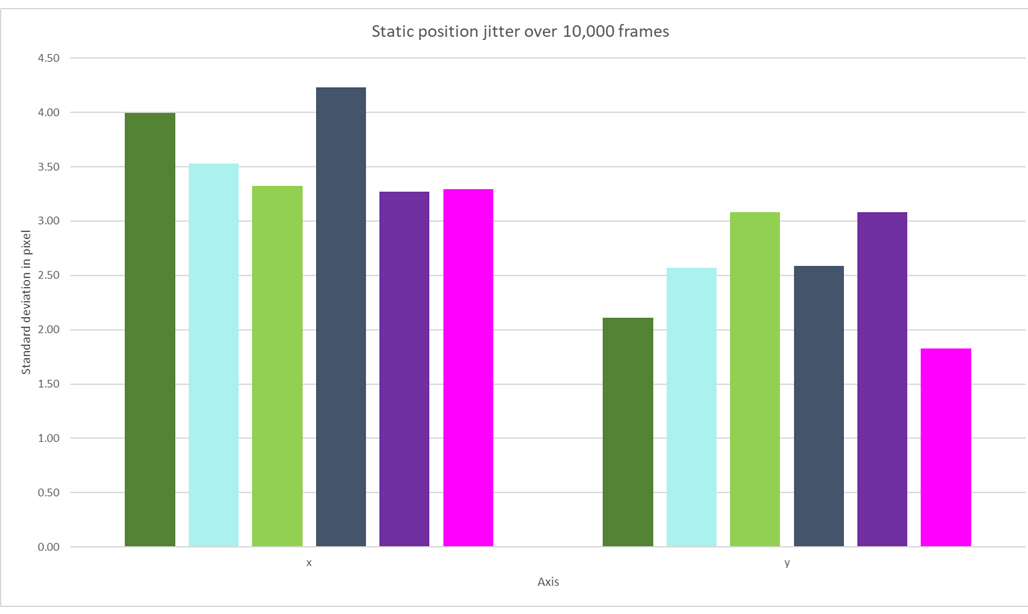
\includegraphics[width=\textwidth]{images/acrylic_color_jitter.jpg}
\caption{Bar chart showing position jitter of final colors in static position}
\label{img:color_jitter}
\end{figure}
 The usage of the acrylic color also provides the least degradation in terms of haptics on the fingers. Figure \ref{img:color_jitter} shows the measured static position jitter of the system with the final colors. The reachable system precision lies between 2 and 5 pixel deviation. At a system resolution of 640x480 pixels, this results in a deviation of $\sim 0.7\%$ on the x axis and $\sim 1.0\%$ deviation on the y axis.
 \newpage
\subsection{Depth measurement accuracy}
To determine the accuracy of the system, the camera rig was aligned horizontally and fixed to a test bench. A large sized colored marker (75 mm x 50 mm) was used as tracking target. The marker was positioned at altering distances from the camera rig along the central axis. The height at which the camera rig is positioned in the experiment setup will be around 100 cm, so the measured distances started at 100 cm from the camera and were decremented in steps of 5 cm until 20 cm in front of the camera rig (see Table \ref{tbl:Depth measurement Values} and Figure \ref{char:DisparityToDistanceChart}).\\
\begin{figure}[H]
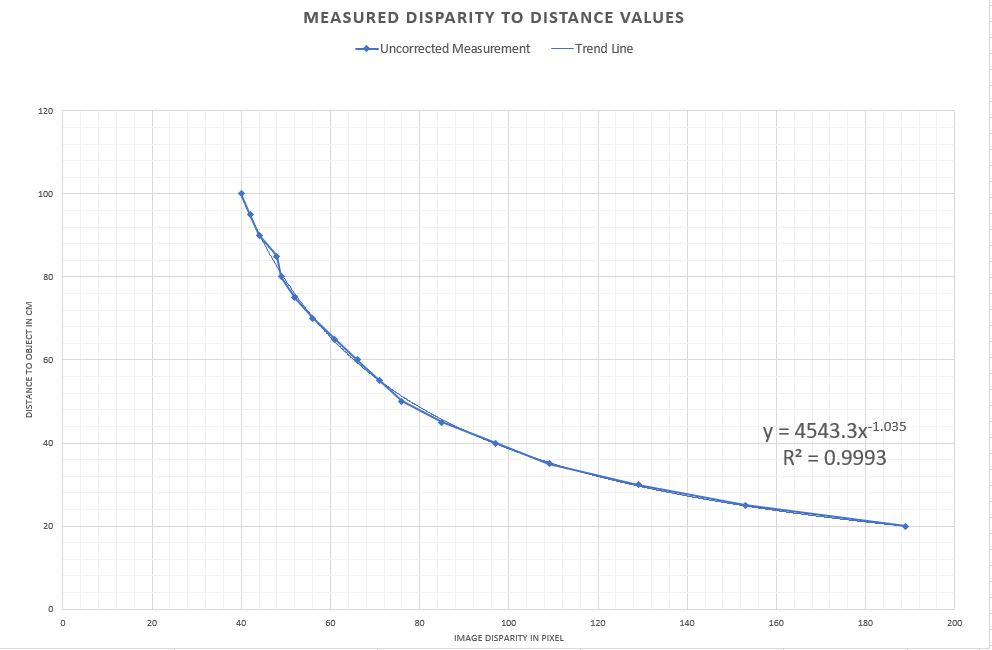
\includegraphics[width=\textwidth]{images/Disparity_to_distance.JPG}
\caption{Chart showing the results of the disparity measurement with a plotted trend line}
\label{char:DisparityToDistanceChart} 
\end{figure}
The accuracy of the camera system is limited by the number of pixels in relation to the camera view angle \cite{JernejMrovlje.2008}:\\
\begin{equation}
\Delta\varphi=\frac{\varphi_0}{x_0}
\end{equation}
\\
For the system setup of $x_{0}=$ 640 px image width and a horizontal view angle of $\varphi_{0}=62.5^\circ$, $\Delta\varphi$ is equal to $0.0977\frac{1^\circ}{pixel}$.\\\\
The resulting distance error would be:\\
\begin{equation}
\frac{\tan \varphi}{\tan(\varphi -\Delta\varphi)}=\frac{\Delta D+D}{D}
\end{equation}\\
\begin{equation}
\label{equ:delta_d}
\Delta D=\frac{D^{2}}{B} tan(\Delta\varphi)
\end{equation}
\\The system error for a target distance $D=100cm$ would therefore result in about $2cm$ of possible error.
As the measured values show deviations of up to $5\%$ from the correct value, the function from the fitted trend line displayed in Figure \ref{char:DisparityToDistanceChart} was taken as a correcting factor for the depth calculation.
\\\\Equation \ref{equ:delta_d} uses the uncorrected values for the calculation. Values lying on the trend line of Figure \ref{char:DisparityToDistanceChart} should correspond more to the correct distance values \cite{ManafA.Mahammed.2013}. The equation can be rewritten to:
\begin{equation}
\label{equ:power_function}
D=k*x^{z}
\end{equation}
with K being:
\begin{equation}
k=\frac{Bx_0}{2\tan(\frac{\varphi_0}{2}+\phi)}
\end{equation}
and \textit{x} the disparity in pixels.
The $\phi$ term in the equation above is used as a compensation for possible alignment errors.
The trend line, which is fit to the measurements in Figure \ref{char:DisparityToDistanceChart} represents the the function needed to fulfill Equation \ref{equ:power_function}. The calculated values are $k=4543.3$ and $z=-1.035$.
With the utilization of the corrected value formula, the accuracy of the depth measurement results is acceptable for the prototype application. For future work, the distance measurement procedure could be applied with more measurement points to refine the resulting function for more precision. The measurement values that were retrieved can be found in Table \ref{tbl:Depth measurement Values}.
\newpage
\begin{landscape}
\begin{table}[]
\label{char:Depth calibration measurement}
\centering
\caption{Depth measurement values}
\label{tbl:Depth measurement Values}
\begin{tabular}{|c|c|c|c|c|c|c|c|}
\hline
\begin{tabular}[c]{@{}c@{}}Real distance \\ from camera (cm)\end{tabular} & \begin{tabular}[c]{@{}c@{}}Left camera\\ x-value\end{tabular} & \begin{tabular}[c]{@{}c@{}}Right camera\\ x-value\end{tabular} & \begin{tabular}[c]{@{}c@{}}Disparity in\\  pixels\end{tabular} & \begin{tabular}[c]{@{}c@{}}Calculated distance\\ in cm\end{tabular} & Deviation in \%(abs.) & Corrected values & Deviation in \%(abs.) \\ \hline
100                                                                       & 302                                                           & 342                                                            & 40                                                             & 99.463                                                              & 0.54                  & 99.670           & 0.33                  \\ \hline
95                                                                        & 301                                                           & 343                                                            & 42                                                             & 94.727                                                              & 0.29                  & 94.760           & 0.25                  \\ \hline
90                                                                        & 300                                                           & 344                                                            & 44                                                             & 90.421                                                              & 0.47                  & 90.304           & 0.34                  \\ \hline
85                                                                        & 298                                                           & 346                                                            & 48                                                             & 82.886                                                              & 2.49                  & 82.523           & -2.91                 \\ \hline
80                                                                        & 296                                                           & 345                                                            & 49                                                             & 81.194                                                              & 1.49                  & 80.780           & 0.98                  \\ \hline
75                                                                        & 296                                                           & 348                                                            & 52                                                             & 76.510                                                              & 2.01                  & 75.960           & 1.28                  \\ \hline
70                                                                        & 293                                                           & 349                                                            & 56                                                             & 71.045                                                              & 1.49                  & 70.349           & 0.5                   \\ \hline
65                                                                        & 289                                                           & 350                                                            & 61                                                             & 65.222                                                              & 0.34                  & 64.388           & 0.94                  \\ \hline
60                                                                        & 289                                                           & 355                                                            & 66                                                             & 60.281                                                              & 0.47                  & 59.344           & 1.09                  \\ \hline
55                                                                        & 286                                                           & 357                                                            & 71                                                             & 56.036                                                              & 1.88                  & 55.022           & 0.04                  \\ \hline
50                                                                        & 285                                                           & 361                                                            & 76                                                             & 52.349                                                              & 4.7                   & 51.279           & 2.56                  \\ \hline
45                                                                        & 280                                                           & 365                                                            & 85                                                             & 46.806                                                              & 4.01                  & 45.668           & 1.48                  \\ \hline
40                                                                        & 265                                                           & 362                                                            & 97                                                             & 41.016                                                              & 2.54                  & 39.831           & 0.42                  \\ \hline
35                                                                        & 258                                                           & 367                                                            & 109                                                            & 36.5                                                                & 4.29                  & 35.300           & 0.86                  \\ \hline
30                                                                        & 244                                                           & 373                                                            & 129                                                            & 30.841                                                              & 2.80                  & 29.650           & 1.17                  \\ \hline
25                                                                        & 288                                                           & 381                                                            & 153                                                            & 26.003                                                              & 4.01                  & 24.848           & 0.61                  \\ \hline
20                                                                        & 206                                                           & 395                                                            & 189                                                            & 21.050                                                              & 5.25                  & 19.965           & 0.17                  \\ \hline
\end{tabular}

\end{table}
\end{landscape}
\section{Data filtering}
The finger marker base jitter measurements showed that the systems can only supply a certain stability of position tracking. This results in the fluctuation of the measurement results. When rendering this unfiltered data directly, a large optical jitter in all positions is the case. Jittering of position values also causes the height calculation algorithm to generate incorrect height values.\\
To counter this data jitter, the incoming data-set is filtered on the "Master" in several steps with the \textit{1 euro filter} presented by Casiez et al. \cite{Casiez.2012}. It uses a first order low-pass filter with an adaptive cutoff frequency to filter noisy signals for high precision and responsiveness. This means that at low speeds, a low cutoff reduces jitter at the expense of lag. At high speeds, the cutoff is increased to reduce lag rather than jitter.\\
The filter was chosen, beacuase of a relative simple and easy implementation as well as an uncomplicated setup and tuning process. It also produces faster and better results in comparsion to the normally used \textit{Kalman filter} \cite{Welch.2001}, \textit{moving average filter} or \textit{low-pass filters and exponential smoothing filters} \cite{LaViola.2003}.\\ The filter needs three base values to function correctly. The first one is the frequency at which the data values are delivered. This can easily be measured from the time stamp differences of the incoming data packages. The other two values are the minimum cutoff frequency$f_{c_{min}} $ of the low pass filter and the slope of the filter curve $\beta$.
\\These values have to be calibrated in a manual process for each marker. In the first step the value of $f_{c_{min}} $ is set to one and $\beta$ is set to zero. The markers are held in a static position or moved very slowly to check for jitter. The value of $f_{c_{min}} $ is then adapted to a point where the jitter is minimized without creating to much lag for these slow movements. In the second step, the tracker is moved fast and the $\beta$ value is increased until lag for fast movements is minimized.
\\\\ In a first step, the incoming data for each finger and the base marker are filtered separately and component-wise. This allows for specific fine tuning of the filter values, as each marker shows different jitter. The incoming values are also passed to the depth calculation algorithm where the z position of the respective marker is calculated. The result is also filtered before all components are written into the final result position vector.\\
The individual filter application to all values resulted in a much smoother and less jittering optical result in comparison to the raw tracking values.
\newpage
\section{Inverse kinematics algorithm}
Figure \ref{img:hand-constraint_debug_view} shows the a debugging representation of the used kinematic structure of the \textit{Caliko} framework. The non-black colored lines of the left picture show the kinematic chains for each finger. The black colored lines are used as an offset structure from the hand base marker.
The kinematic chains all have their own target point for which the algorithm can solve for. All chains are grouped into a kinematic model for easier data handling. The kinematic model provides a container for easier access of the base and the connection structure through which the fingers are connected to the base.
With this data, the algorithm is capable of calculating a solution for each kinematic finger chain and applying these values to the position. If the target is reachable, the digital finger position should match the pose of its real world counterpart up to a specified threshold value.
\begin{figure}[H]
\centering
\includegraphics[width=0.5\textwidth]{images/hand_model_combo.png}
\caption{Hand model representation of the used IK framework: a) Kinematic chains and base structure, b) Hand model with visualized movement constraints}
\label{img:hand-constraint_debug_view} 
\end{figure}
The right image shows the same model with applied constraints to each chains. The framework differentiates between base-bone constraints and normal bone constraints. The base-bone constraints are treated separately as the base-bone is the starting point of the kinematic chain and therefore effects all following bones. In the 3D mode constraints with either a global or a local reference axis can be applied. The local reference axis usually refers to a axis of the previous bone. Global constraints are used for base-bone constraints. The reference axis can the be used for the specific type of constraint. The framework supports hinge type constraints and rotor constraints. The hinge types define a rotation axis around which the bone can rotate (1 DOF). The rotor-based constraint defines an angle for a cone on a defined axis which limits the movement of the joint in multiple directions (2 DOF). This circular curve limitation is a downside of the framework as a parabolic curve description for a rotor-based constraint would better fit the movement capabilities of the fingers.
\newpage 
\section{Grabbing test}
To test the tracking limitations of the system , a grabbing test with the tracked \textit{HTC Vive} marker and the tracked hand was done.
Before the test was started, it was ensured that the infrared signals from the object tracker do not interfere with the camera images for tracking. 
\begin{figure}[H]
\centering
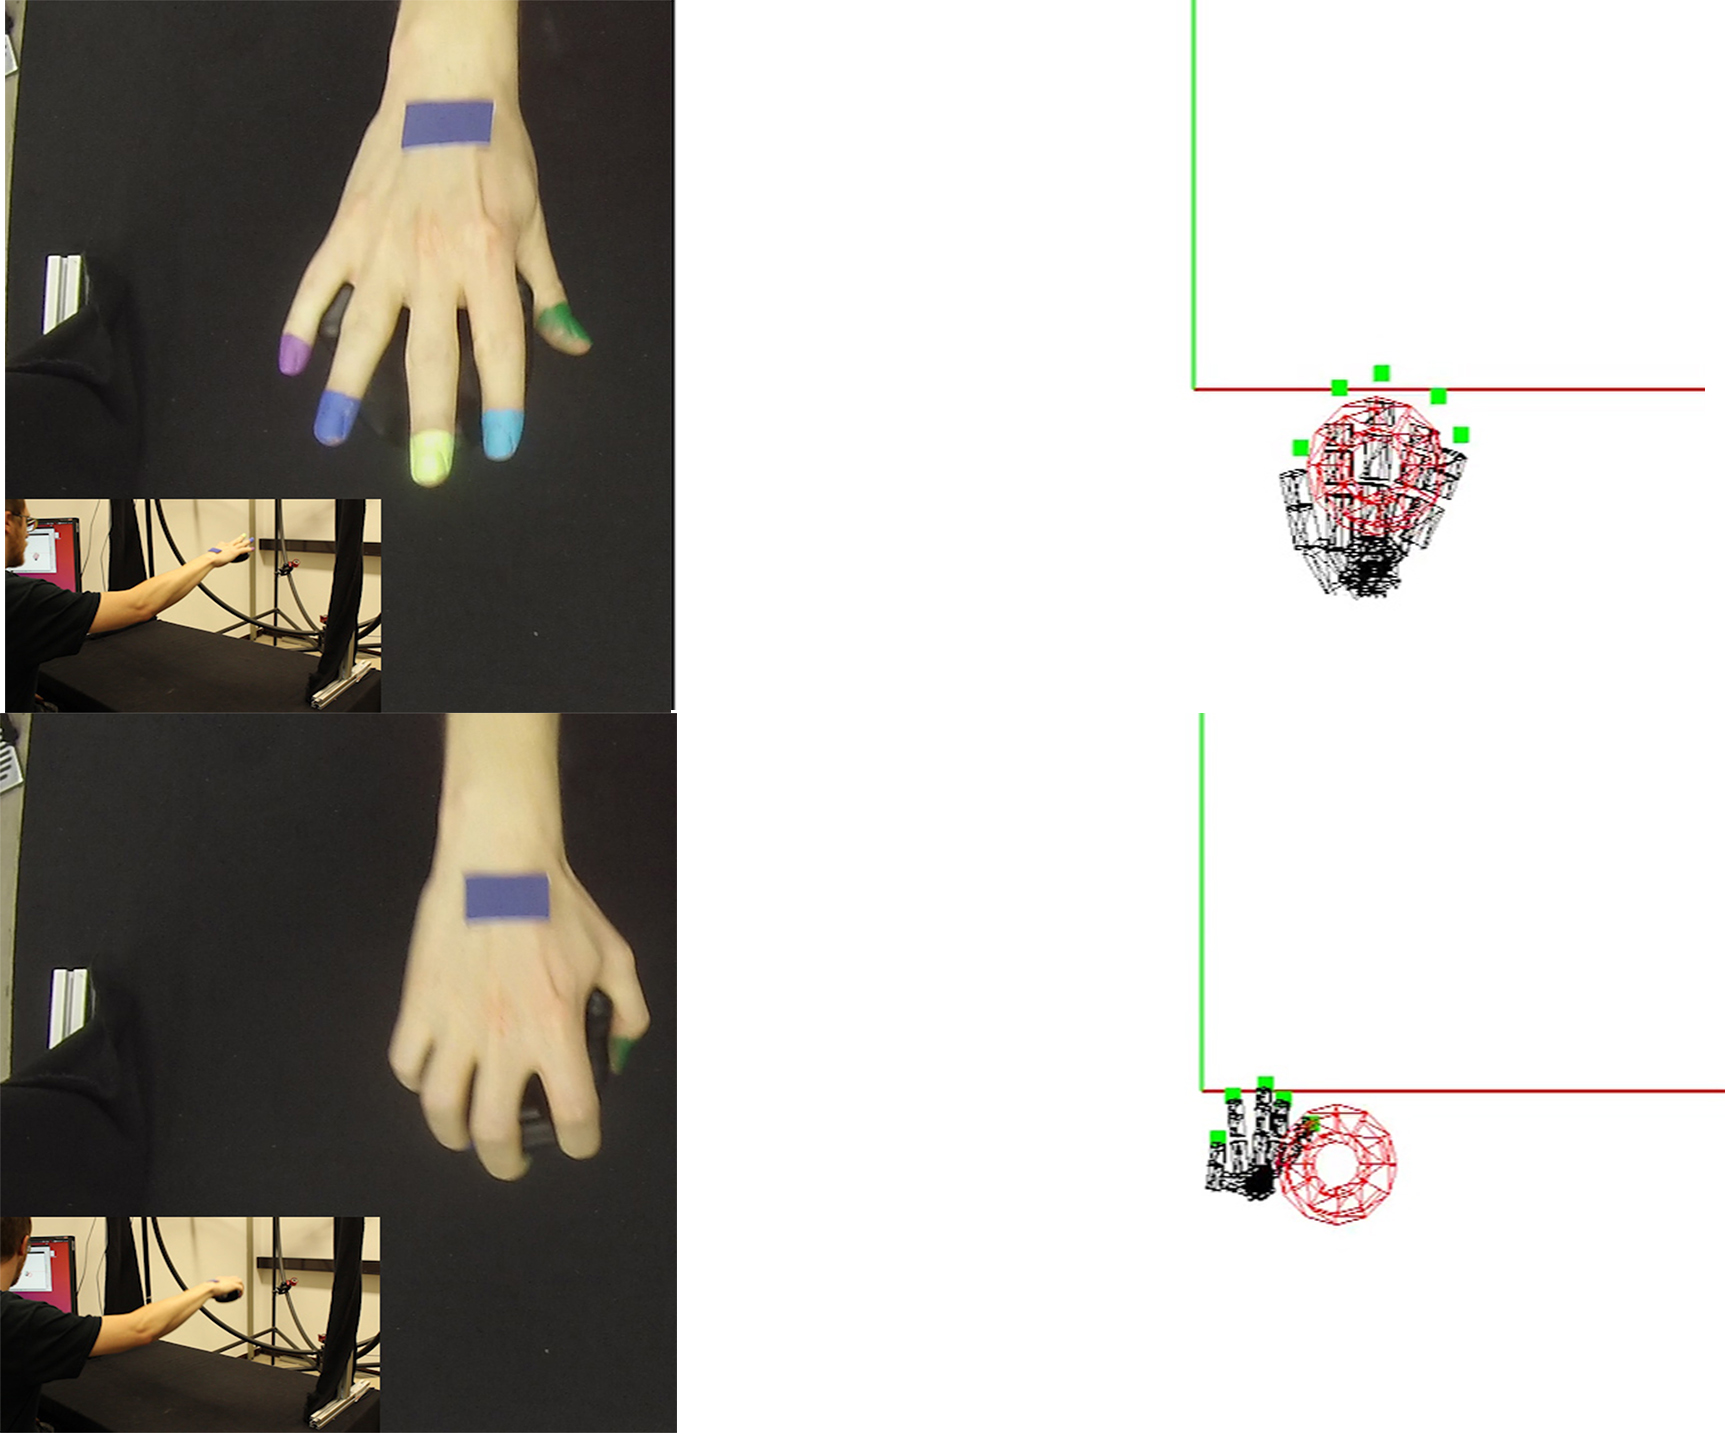
\includegraphics[width=0.8\textwidth]{images/occlusion_set.jpg}
\caption{Grabbing test results: Upper image pair shows grabbing of tracker without finger occlusion. The position of the hand and the fingers is correct. The bottom image pair shows the mentioned marker occlusion problem. The tracker  position is correct but the finger tracking is lost and the positoin of the hand incorrect.}
\label{img:hand_rendering}
\end{figure}
The built-in infrared filters of the camera manage to filter out the signals, as no image distortion was visible. The test chore was to pick up the tracked marker based on the position of the marker representation in digital space.
A precise initial position calibration for the object tracker is done to ensure matching real and digital positions. The tracking limitations of the system showed when bending the fingers around the marker to pick it up. The bending causes the fingers to be occluded from the cameras and no new position can be tracked. This occlusion problem results from the positioning of the cameras. The top-down view limits the movement areas of the hand where all fingers markers can be tracked. The hand position marker is not affected from this occlusion problem as long as the hand is not turned around.
For the system to handle grabbing movements correctly, the cameras would have to be positioned at a different angle than the top down-view or a further pair of cameras recording from a different angle has to be added.

\newpage
\chapter{Resume}

Future work:\\
-improve depth tracking value preciion through a more elaborate calibration seesion where the depth correcton algorith is further optimized
\\
-improve image reading source code to accept hgher framerates. The hardware capacbilities provide image reading frequences of up to 90fps, current bottleneck is the c++ implementaion which only provides 30 fps max.
\\
-When utilizng higher framerates, the multiproceesng approach will be viable to gain performance. Optimizaton work on the implementaion can be done.\\
-Image manipulaton on the cpu is rather costly, even at small image sizes. The raspberry Pi has a "small" gpu unit onboard, whch is in dle state when the device is run in headless mode. The gpu could then be utilzed to do heavy weight image calculation such as stereo rectification.\\
-Optimization pont would also be creating a mor optimized verson of the color thresholding algorithm where the threshoding for all of the thracking colors is done in one run on the current frame. It is also to be evaluated if ths problem falls can be expressed as a SIMD functon and would benefit from the processng on the gpu.
\\
The current prototype is still missing an graphcal user interface on the display side. Further communication of states on the slave Pi's to the master unit would also be beneficial.
\\
The habd data that is used for prototyping is still hardcoded and only manually configurable. A calibration procedure for the system as well as a suitable data format for representing and translating these values for the IK algortihm s still to be done.
\\
-Shrnk tubing showed to be a utilzable material for the usecase. Downsinde of the material is that the colors used are the largest spectrum of colors available on the market and geting outer colors is relatively hard. Other materal shuold be evaluated.



\newpage
%Erzeugt ein Abbildungsverzeichnis
\pagenumbering{roman}
	\listoffigures
	%Fügt die Zeile "`Abbildungsverzeichnis"' als Chapter ins Inhaltsverzeichnis ein
	\addcontentsline{toc}{chapter}{Abbildungsverzeichnis}
\newpage
	
	%Erzeugt ein Tabellenverzeichnis
	\listoftables
	%Fügt die Zeile "`Tabellenverzeichnis"' als Chapter ins Inhaltsverzeichnis ein
	\addcontentsline{toc}{chapter}{Tabellenverzeichnis}
\newpage

% To change the title from References to Bibliography:
\renewcommand\refname{Literaturverzeichnis}

%Paket für ein deutsches Literaturverzeichnis

\bibliography{literature} % refers to literatur.bib

	%Fügt die Zeile "`Literaturverzeichnis"' als Chapter ins Inhaltsverzeichnis ein
	\addcontentsline{toc}{chapter}{Literaturverzeichnis}
\newpage

%!TEX root = ../Masterthesis.tex
\chapter*{Eidesstattliche Erklärung}
%\addcontentsline{toc}{chapter}{Eidesstattliche Erklärung}

Ich versichere, die von mir vorgelegte Arbeit selbständig verfasst zu haben.\\ 
Alle Stellen, die wörtlich oder sinngemäß aus veröffentlichten oder nicht veröffentlichten Arbeiten anderer entnommen sind, habe ich als entnommen kenntlich gemacht. Sämtliche Quellen und Hilfsmittel, die ich für die Arbeit benutzt habe, sind angegeben.\\ 
Die Arbeit hat mit gleichem Inhalt bzw. in wesentlichen Teilen noch keiner anderen Prüfungsbehörde vorgelegen.
\vspace{1.5cm}
\\
Köln, xx. August 2016
\vspace{3cm}
\\
Oliver Kalbfleisch


% chapter eidesstattliche_erklärung (end)
\end{document}
